\documentclass[
	letterpaper
	12pt
]{template}

\usepackage{apacite}
\usepackage{titling}
\usepackage[font=footnotesize,labelfont=bf]{caption}

\setlength{\droptitle}{-10em}

\newcommand{\bref}[2]{\textbf{\hyperref[#1]{#2}}}

\title{DC Power Supply}

\author{Sebastien Psarianos, Yuchen Jiang}

\date{\today}



\begin{document}
\maketitle
\section{Abstract}
In this lab report, we examined various ways that alternating current (AC) can be converted into direct current (DC). We explored rectification methods, voltage
smoothing, low pass filters and Zener Diodes and compared their effectiveness using the \bref{eqn::ripple}{Ripple Factor} metric. The best method for rectification that was tested was the bridge rectifier and the lowest ripple factor that we achieved using smoothing techniques was using a zener diode transistor regulation circuit with half-wave rectification. During the course of this study, we determined that to more rigorously compare these conversion methods, we would have to analyze the efficiency of each circuit in addition to their ripple. This would provide a more insightful overview of the real world trade-offs involved in AC to DC conversion.
\section{Introduction}
In this lab we explored the process of converting alternating current (AC) to direct current (DC). Throughout a series of experiments we investigated various rectification methods and explored smoothing and stabilization techniques using capacitors, inductors, Zener diodes and transistors. Each experiment consisted of assembling one AC to DC conversion circuit, using an adjustable transformer to vary the voltage and isolate the circuit from the mains power. Through measuring and calculating inferred voltages and currents using \bref{eqn::ohm}{Ohm's Law} across the circuits, we were able to analyze the quality of the conversion through one key characteristic: \bref{eqn::ripple}{Ripple Factor}. Ripple Factor is a metric that describes the quality of the DC conversion. Note that all \bref{eqn::ripple}{Ripple Factor} and current values' errors were calculated using \bref{prop::div}{Division Propagation}. Sample calculations for both are available in \bref{appdx::A}{Appendix A}
\begin{equation}\label{eqn::ohm}
	\text{Ohm's Law \cite{Rashid_2006}:}\ \ I_{dc}={V_{dc}\over R}
\end{equation}
\begin{equation}\label{eqn::ripple}
	\text{Ripple Factor \cite{Rashid_2006}:} \ \ RF = {V_{ac}\over V_{dc}}
\end{equation}
% \begin{equation}\label{eqn::eff}
% 	\text{Efficiency \cite{Rashid_2006}:} \ \ \nu = {P_{out}\over P_{in}}
% \end{equation}
\begin{equation}\label{eqn::power}
	\text{Power \cite{Rashid_2006}:}\ \  P = IV = {V^2\over R}
\end{equation}
\begin{equation}\label{prop::div}
	\text{Division / Multiplication Propagation:}\ \ \Delta ({x/ y}) = \sqrt{{\Delta x\over x} + {\Delta y\over  y}}
\end{equation}

Out measurements were primarily taken using a Keysight InfiniiVision 1000 X-Series Oscilloscope. We made use of the AC RMS and DC RMS measurements for all of our voltages. The DC RMS measures the raw root mean squared of the signal whereas the AC RMS removes the DC portion of the signal from this calculation, giving a quantitative representation of the ripple in the system \cite{RMS}. In this study we used these tools to compare various strategies of AC to DC conversion detailed in the following sections.

\section{Experiment A}\label{exp::A}
\subsection{Methodology}\label{method::A}
In this experiment, we assembled the half-wave rectifier depicted in \textbf{\hyperref[apparatus::A]{Figure 1}}.
\begin{figure}[H]\label{apparatus::A}
	\centering
	\begin{minipage}[c]{0.4\textwidth}
		\centering
		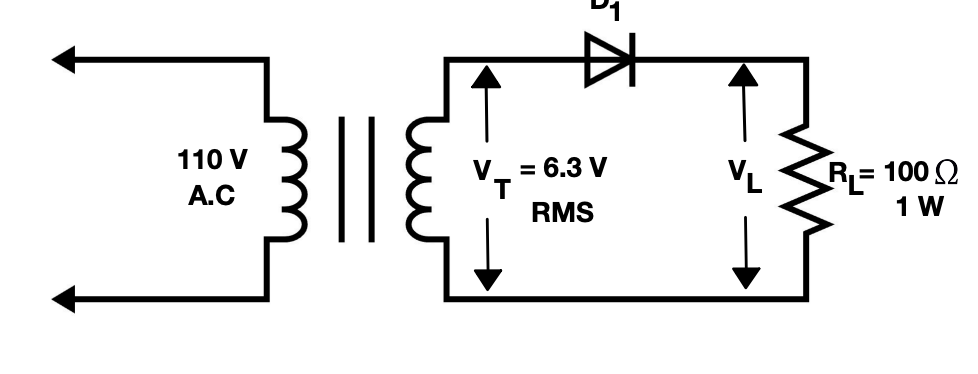
\includegraphics[width=\textwidth]{figures/A/schematic.png}
		\caption{Schematic for experiment A \\ \protect\cite{labManual}}
	\end{minipage}
\end{figure}

The oscilloscope probes were set to measure $V_T$ and $V_L$ on channels 1 and 2 respectively. Both AC and DC RMS voltages were noted down and the data was then saved onto a USB flash drive.

\subsection{Results and Analysis}\label{res::A}
A plot of the oscilloscope readout is pictured in \bref{data::A}{Figure 23} ($V_T$) and \bref{data::A}{Figure 24} ($V_L$) and the RMS voltage measurements are as follows:
\begin{figure}[H]    \centering    \begin{tabular}{|l|c|c|}
        \hline
        Measured Value & AC RMS & DC RMS \\
        \hline
        $V_L$ & $3.64\pm 0.01\unit{V}$ & $4.61\pm 0.01\unit{V}$ \\
        $V_T$ & $7.42\pm 0.01\unit{V}$ & $7.43\pm 0.01\unit{V}$ \\
        \hline
    \end{tabular}    \caption{Oscilloscope measured voltages for experiment A}\end{figure}
The half-wave rectifier performed its intended purpose, inhibiting current flow in one direction, resulting in the bottom half of the waveform being cut off. This gave a strictly non-negative voltage. However, one distinct disadvantage of this system is that during the negative portion of the AC signal, the transformer is doing no work on the resistor. This is reflected in the substantial loss in AC and DC RMS voltage at $V_L$ compared to $V_T$.\\

The ripple factor of this rectifier as defined in \bref{eqn::ripple}{Equation 2} was calculated as: $0.790\pm0.004$. This ripple factor is far below the literature value of 1.21 \cite{Rashid_2006}. Additionally, there is a small drop in the peak voltage between the $V_T$ plot and the $V_L$ plot. This is likely due to the internal voltage-drop of the diode.










\section{Experiment B}\label{exp::B}
\subsection{Methodology}\label{method::B}
In this experiment, we assembled the full-wave rectifier depicted in \textbf{\hyperref[apparatus::B]{Figure 3}}.
\begin{figure}[H]\label{apparatus::B}
	\centering
	\begin{minipage}[c]{0.45\textwidth}
		\centering
		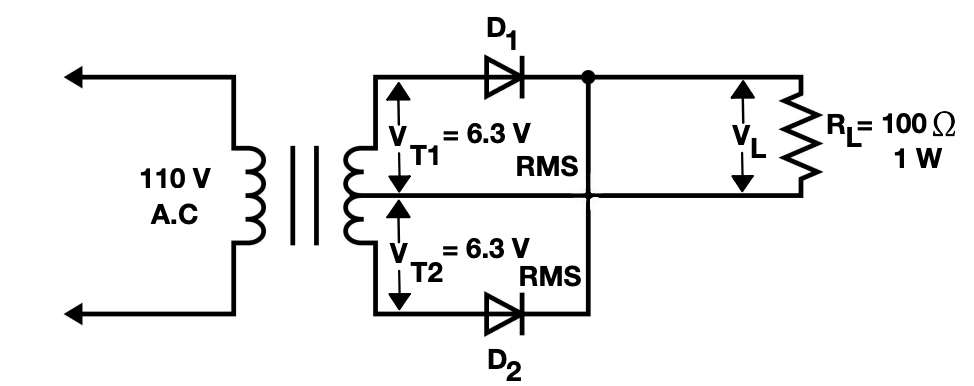
\includegraphics[width=\textwidth]{figures/B/schematic.png}
		\caption{Schematic for experiment B \\ \protect\cite{labManual}}
	\end{minipage}
\end{figure}

The oscilloscope probes were set to measure $V_{T1}$ and $V_L$ on channels 1 and 2 respectively. The waveforms were scaled appropriately. After noting down the DC and AC RMS voltages for both values, the data was then saved onto a USB flash drive. Channel 1 was then changed to $V_{T2}$ and the same procedure was followed.

\subsection{Results and Analysis}
The oscilloscope readouts from the first configuration are shown in \bref{data::B}{Figure 25} ($V_{T1}$) and \bref{data::B}{Figure 26} ($V_L$). The readouts for the second configuration are shown in \bref{data::B2}{Figure 27} ($V_{T2}$) and \bref{data::B2}{Figure 28} ($V_L$). The measured RMS voltage values are as follows:

\begin{figure}[H]    \centering    \begin{tabular}{|l|c|c|}
        \hline
        Measured Value & AC RMS & DC RMS \\
        \hline
        $V_{L}$ & $3.10\pm 0.01\unit{V}$ & $6.51\pm 0.01\unit{V}$ \\
        $V_{L}$ & $3.11\pm 0.01\unit{V}$ & $6.51\pm 0.01\unit{V}$ \\
        $V_{T1}$ & $7.40\pm 0.01\unit{V}$ & $7.40\pm 0.01\unit{V}$ \\
        $V_{T2}$ & $7.39\pm 0.01\unit{V}$ & $7.39\pm 0.01\unit{V}$ \\
        \hline
    \end{tabular}    \caption{Oscilloscope measured voltages for experiment B}\end{figure}

The full-wave rectifier allows both the positive and negative voltage from the $AC$ signal from $V_T$ to be converted to positive voltage in $V_L$. This allows more of the input potential to not be wasted when compared to \bref{exp::A}{Experiment A}. This is clearly shown in the difference from $V_{T1,DCRMS} \rightarrow V_{L,DCRMS}$ between the two experiments.\\

The ripple factor of the full wave rectifier is $0.477\pm0.002$.
This is very close to the literature value of 0.482 \cite{Rashid_2006}. Additionally, the same voltage peak drop that was seen in \bref{exp::A}{Experiment A} is present here. This is again likely due to voltage drop from the diode.







\section{Experiment C}\label{exp::C}
\subsection{Methodology}\label{method::C}
In this experiment, we assembled the bridge rectifier depicted in \textbf{\hyperref[apparatus::C]{Figure 5}}.

\begin{figure}[H]\label{apparatus::C}
	\centering
	\begin{minipage}[c]{0.45\textwidth}
		\centering
		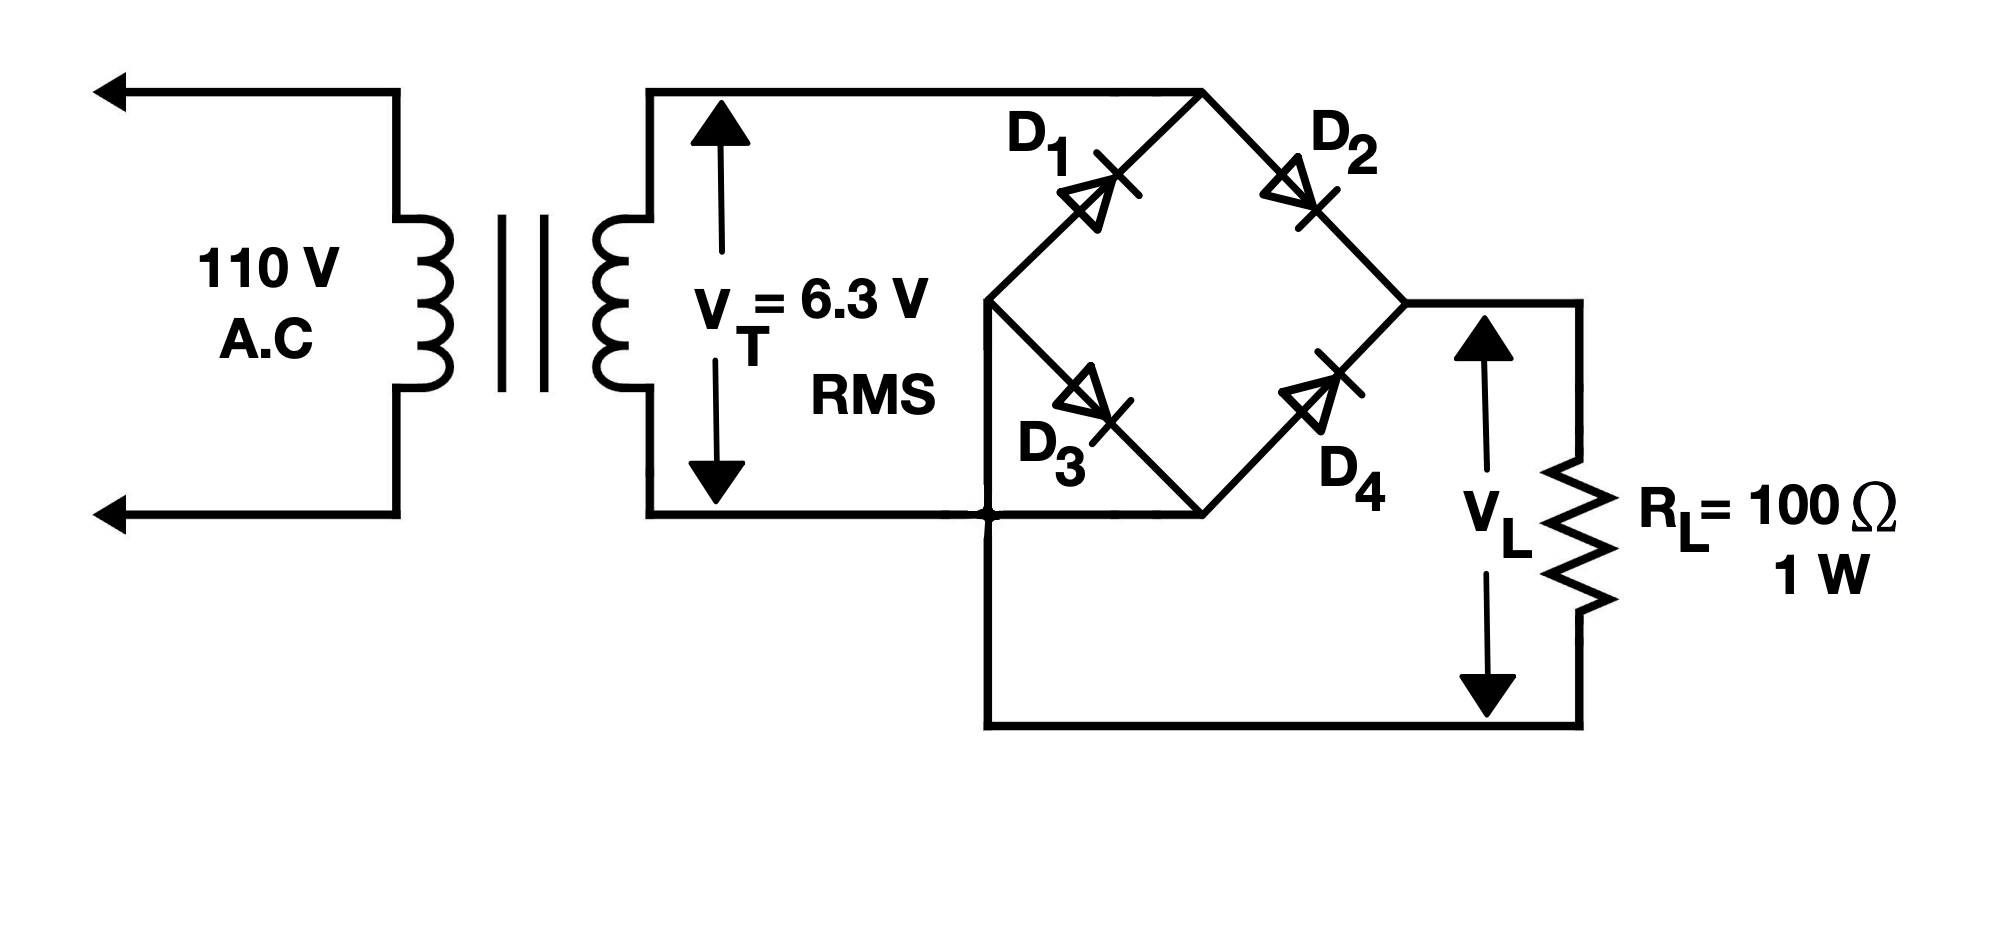
\includegraphics[width=\textwidth]{figures/C/schematic.png}
		\caption{Schematic for experiment C}
	\end{minipage}
\end{figure}

The oscilloscope probe for channel 1 was set to measure $V_L$. The DC and AC RMS voltage values were noted down. Then the data was saved to a USB flash drive. Channel 1 was then set up to measure $V_T$ and the same procedure was followed again. Both measurements had to be done separately due to the lack of a common ground on the bridge rectifier.

\subsection{Results and Analysis}
For experiment C, the oscilloscope readouts from the first configuration are shown in \bref{data::C}{Figure 29} ($V_{L}$).The readouts for the second configuration are shown in \bref{data::B2}{Figure 30} ($V_{T}$). The measured AC and DC RMS voltages are as follows:\\

\begin{figure}[H]    \centering    \begin{tabular}{|l|c|c|}
        \hline
        Measured Value & AC RMS & DC RMS \\
        \hline
        $V_{L}$ & $3.00\pm 0.01\unit{V}$ & $5.90\pm 0.01\unit{V}$ \\
        $V_{T}$ & $7.35\pm 0.01\unit{V}$ & $7.35\pm 0.01\unit{V}$ \\
        \hline
    \end{tabular}    \caption{Oscilloscope measured voltages for experiment C}\end{figure}
This resulted in a similar oscilloscope plot to the full-wave rectifier. There was again a drop in peak voltage when comparing $V_T$ and $V_L$, however this time it seems to be about twice as much as the half and full-wave rectifier. This is likely due to the fact that any complete loop of the circuit will go through at least two diodes. However, for the half and full-wave rectifier, this is only one diode.\\\\
The \bref{eqn::ripple}{Ripple Factor} of this circuit is $0.509\pm0.002$. This is quite close to the literature value of 0.48 \cite{Rashid_2006}.








\section{Experiment D}\label{exp::D}
\subsection{Methodology}
In this experiment, we assembled the smoothing circuit depicted in \textbf{\hyperref[apparatus::D]{Figure 7}}.
\begin{figure}[H]\label{apparatus::D}
	\begin{minipage}[c]{0.45\textwidth}
		\centering
		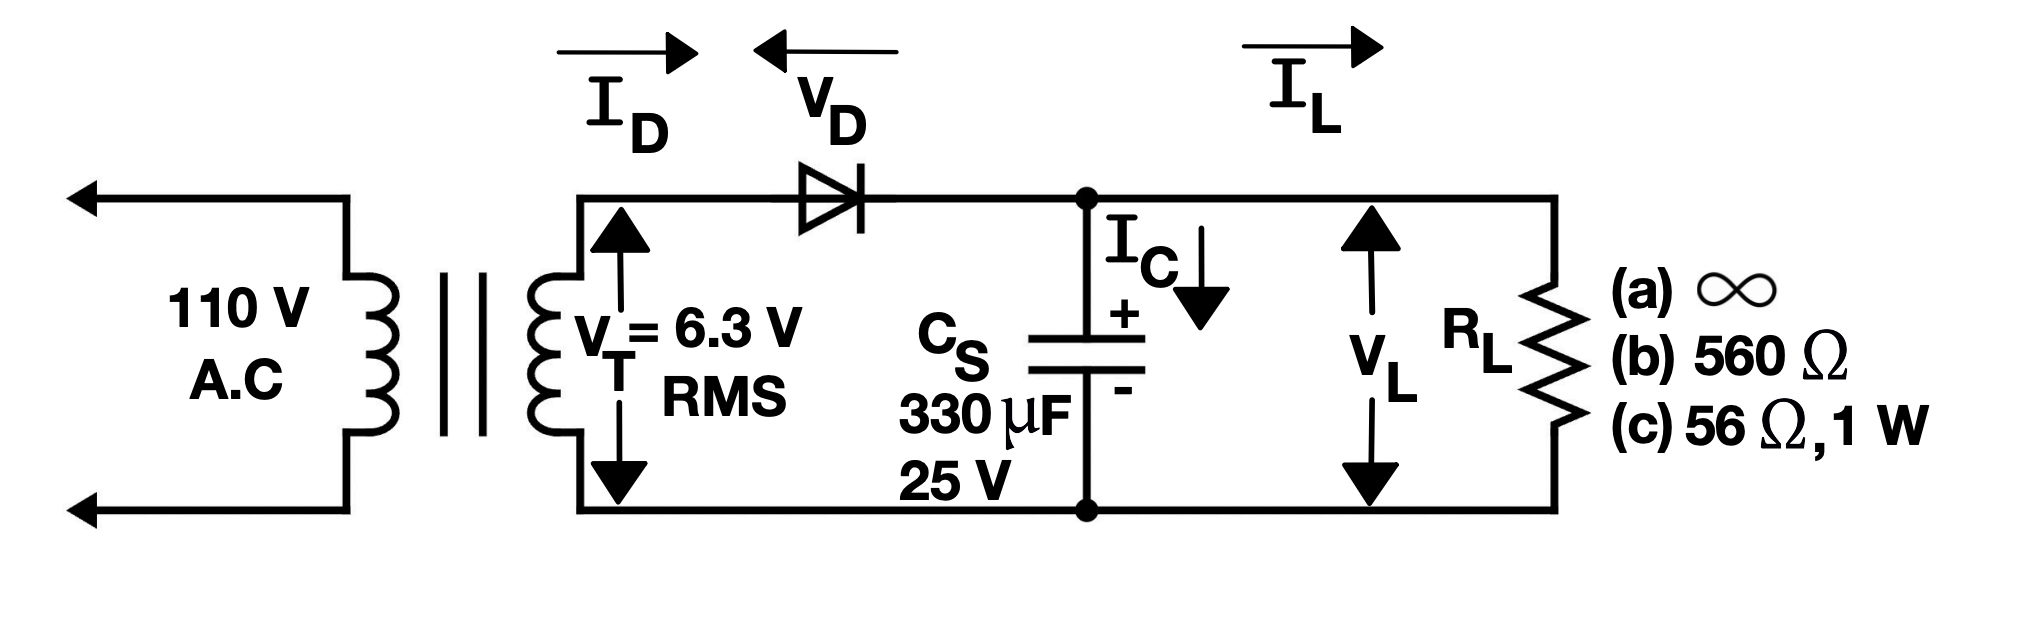
\includegraphics[width=\textwidth]{figures/D/schematic.png}
		\caption{Schematic for experiment D \\ \protect\cite{labManual}}
	\end{minipage}
	\hfill
	\begin{minipage}[c]{0.45\textwidth}
		\centering
		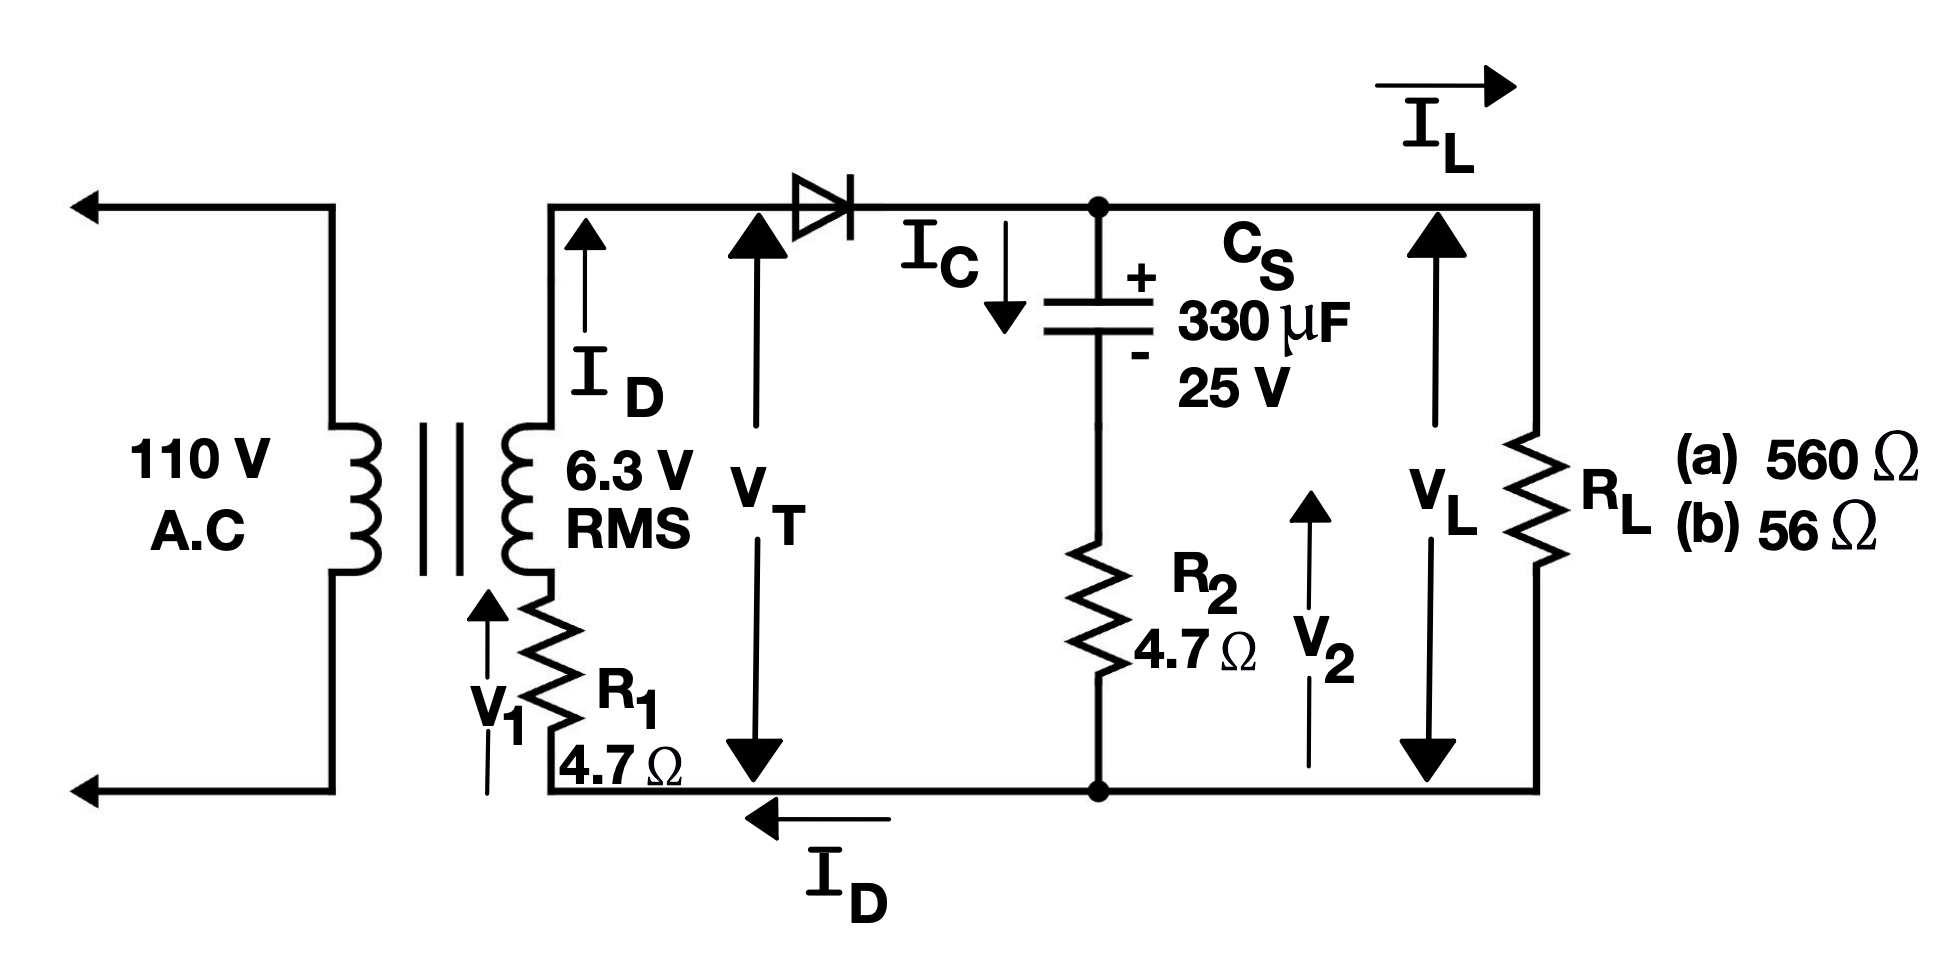
\includegraphics[width=\textwidth]{figures/D/schematic2.png}
		\caption{Schematic 2 for experiment D \\ \protect\cite{labManual}}
	\end{minipage}
\end{figure}
\subsubsection{Part 1}\label{method::D1}
For each of the resistance values shown in \textbf{\hyperref[apparatus::D]{Figure 8}}, we set up the oscilloscope with $V_L$ on channel 1 and $V_T$ on channel 2. Then we noted down the AC and DC RMS values of $V_L$ and $V_T$. We then saved the data onto a USB flash drive. Note that $\infty$ resistance was simulated using a large $2.7k\Omega$ resistor.
\subsubsection{Part 2}\label{method::D2}
In the second part of this experiment, we altered the circuit to contain the resistors shown in \textbf{\hyperref[apparatus::D]{Figure 8}}. The oscilloscope was used to measure DC and AC RMS voltages for $V_1, V_2, V_3$ for both $R_L = 560\Omega, 56\Omega$. All of these measurements were noted down and saved to a USB flash drive.



\subsection{Results and Analysis}
{\subsubsection{Part 1}}
For Part 1 of Experiment D, the oscilloscope readouts are shown in figures \bref{data::D}{31} $\rightarrow$ \bref{data::D3}{36}. The measured voltage values are as follows:
\begin{figure}[H]    \centering    \begin{tabular}{|l|c|c|}
        \hline
        Measured Value & AC RMS & DC RMS \\
        \hline
        $V_{L} - 2.7\unit{k\ohm}$ & $No Edges$ & $No Edges$ \\
        $V_{L} - 560\unit{\ohm}$ & $240\pm 10\unit{mV}$ & $8.94\pm 0.01\unit{V}$ \\
        $V_{L} - 56\unit{\ohm}$ & $1.37\pm 0.01\unit{V}$ & $6.14\pm 0.01\unit{V}$ \\
        $V_{T} - 2.7\unit{k\ohm}$ & $7.49\pm 0.01\unit{V}$ & $7.49\pm 0.01\unit{V}$ \\
        $V_{T} - 560\unit{\ohm}$ & $7.42\pm 0.01\unit{V}$ & $7.42\pm 0.01\unit{V}$ \\
        $V_{T} - 56\unit{\ohm}$ & $6.99\pm 0.01\unit{V}$ & $7.00\pm 0.01\unit{V}$ \\
        \hline
    \end{tabular}    \caption{Oscilloscope measured voltages for experiment D Part 1}\end{figure}
In the case of the  $2.7\unit{k \ohm}$ resistor there were no edges on $V_L$, making it impossible to measure the ripple factor. This is reflected in the oscilloscope plots in \bref{data::D}{Figure 32} ($V_T$) and \bref{data::D}{Figure 31} ($V_L$), $V_L$ seems to be essentially just noise around the $9.75\unit{V} \rightarrow 10.10\unit{V}$ range. Therefore, a graphical analysis is not possible.\\\\
For the $560\unit{\ohm}$ resistor, inspecting the oscilloscope plots in \bref{data::D2}{Figure 33} ($V_T$) and \bref{data::D2}{Figure 34} ($V_L$), it is clear that the rectification was successful in providing a non-negative voltage. Additionally, the capacitor smoothing produced a wave amplitude in the sub $0.5\unit{V}$ range. Comparing this to the rectification circuits in experiments A, B and C where the voltage periodically approached $0V$, this is a much closer approximation to a DC signal. This is reflected in the ripple factor of $0.026\pm 0.001$, which is substantially lower than any of the previously explored rectification methods. \\\\
In the oscilloscope plots for the $56\unit{\ohm}$ resistor (\bref{data::D3}{Figure 35} ($V_T$) and \bref{data::D3}{Figure 36} ($V_L$)), the waveform is similar in shape to the $560\unit\ohm$ resistor previously tested. One notable difference is that the amplitude is higher in this experiment. This is also shown in the ripple factor of $0.214\pm 0.02$ which is much higher than the $56\unit{\ohm}$ resistor, suggesting that the lower resistance $R_L$ value lead the capacitor smoothing to be less effective. This could be due to the lower resistance allowing the capacitor to discharge too quickly to smooth the circuit sufficiently. Although, it can be noted that the ripple factor is still significantly better than the half-wave rectifier alone.

\subsubsection{Part 2}
For Part 2 of Experiment D, the oscilloscope readouts are shown in figures \bref{data::D4}{Figure 37} $\rightarrow$ \bref{data::D6}{Figure 42}. The measured voltage values are as follows:
\begin{figure}[H]    \centering    \begin{tabular}{|l|c|c|}
        \hline
        Measured Value & AC RMS & DC RMS \\
        \hline
        $V_{1} - 560\unit{\ohm}$ & $170\pm 10\unit{mV}$ & $190\pm 10\unit{mV}$ \\
        $V_{1} - 56\unit{\ohm}$ & $660\pm 10\unit{mV}$ & $780\pm 10\unit{mV}$ \\
        $V_{2} - 560\unit{\ohm}$ & $150\pm 10\unit{mV}$ & $160\pm 10\unit{mV}$ \\
        $V_{2} - 56\unit{\ohm}$ & $560\pm 10\unit{mV}$ & $560\pm 10\unit{mV}$ \\
        $V_{L} - 560\unit{\ohm}$ & $230\pm 10\unit{mV}$ & $8.24\pm 0.01\unit{V}$ \\
        $V_{L} - 56\unit{\ohm}$ & $920\pm 10\unit{mV}$ & $4.70\pm 0.01\unit{V}$ \\
        \hline
    \end{tabular}    \caption{Oscilloscope measured voltages for experiment D Part 2}\end{figure}
Using the equations for \bref{eqn::ohm}{Ohm's Law}, \bref{eqn::ripple}{Ripple Factor} and \bref{prop::div}{Division Propogation} we calculated the currents $I_1$ and $I_2$ as well as the ripple factor for both the $560\unit\ohm$ and $56\unit\ohm$ resistor.\\\\
For $R_L = 560\unit\ohm$ the calculated values are: $I_1= 0.040 \pm 0.002 \unit{A}$, $I_2= 0.033 \pm 0.002 \unit{A}$,  $RF=0.028\pm0.001$. \\\\
For $R_L = 56\unit\ohm$ the calculated values are: $I_1= 0.165 \pm 0.002 \unit{A}$, $I_2= 0.118 \pm 0.002 \unit{A}$, $RF= 0.196\pm0.002$


\section{Experiment E}\label{exp::E}
\subsection{Methodology}\label{method::E}
In this experiment, the low-pass filter circuit depicted in \textbf{\hyperref[apparatus::E]{Figure 11}} was assembled. Note that a $1.5\unit{H}$ inductor was used at $L$.
\begin{figure}[H]\label{apparatus::E}
	\centering
	\begin{minipage}[c]{0.45\textwidth}
		\centering
		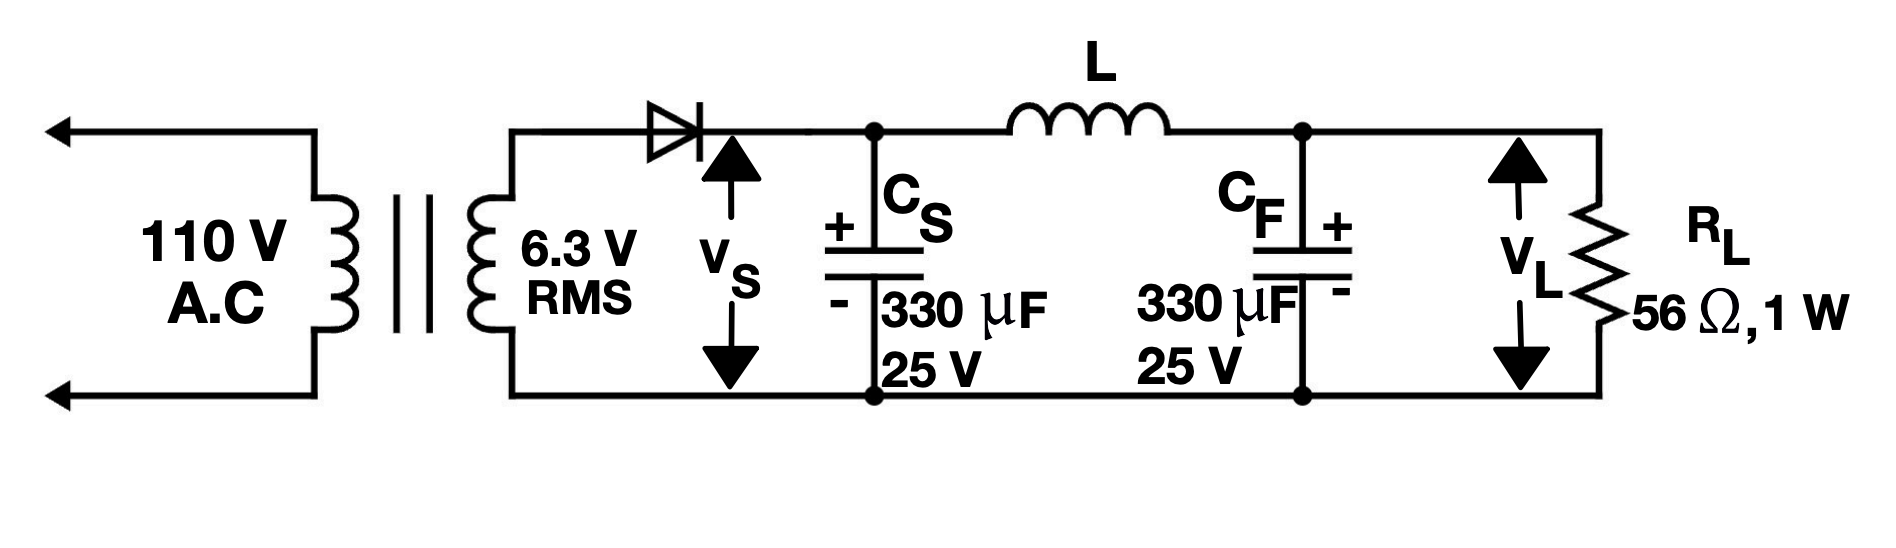
\includegraphics[width=\textwidth]{figures/E/schematic.png}
		\caption{Schematic for experiment E \\ \protect\cite{labManual}}
	\end{minipage}
\end{figure}
We set up the oscilloscope probes to measure $V_S$ on channel 1 and $V_L$ on channel 2. We measured the AC and DC RMS values of both voltages, exporting the data onto a USB flash drive. Then, the oscilloscope was set to the AC coupling and this data was then also exported onto a USB flash drive.


\subsection{Results and Analysis}
The measured voltage values were:\\
\begin{figure}[H]    \centering    \begin{tabular}{|l|c|c|}
        \hline
        Measured Value & AC RMS & DC RMS \\
        \hline
        $V_{L}$ & $1.11\pm 0.01\unit{V}$ & $6.92\pm 0.01\unit{V}$ \\
        $V_{S}$ & $20\pm 10\unit{mV}$ & $4.59\pm 0.01\unit{V}$ \\
        \hline
    \end{tabular}    \caption{Oscilloscope measured voltages for experiment E}\end{figure}

The calculated ripple factor was $0.005 \pm 0.002\unit{V}$. This is the lowest that has been achieved thus far, significantly lower than both of the measurable experiments from \bref{exp::D}{Experiment D}. This is reflected in the very low amplitudes of the waves in the oscilloscope readouts for $V_L$ in figures \bref{data::E}{Figure 43} and \bref{data::E2}{Figure 44}. \\\\
The $V_S$ measurements in figures \bref{data::E}{Figure 44} and \bref{data::E2}{Figure 46} are both essentially just the same waveform from \bref{exp::D}{Experiment D}, however with a different amplitude. This makes sense seeing as the measurement $V_S$ is essentially the same potential as the $V_L$ in \bref{data::E2}{Figure 44} and \bref{data::E2}{Figure 46}\\\\
The transition from the DC coupling in figures \bref{data::E}{43} and \bref{data::E}{44} to the AC coupling in \bref{data::E2}{45} and \bref{data::E2}{46} didn't seem to have much of an effect on the readout.






\section{Experiment F}\label{exp::F}
\subsection{Methodology}\label{method::F}
The Zener diode is specifically designed to keep a voltage across its terminals when its, in bias. To test this property we will vary the line supply voltage and load resistance ($R_L$). By doing we can observe how the Zener diode responds to changes in input voltage and load conditions. In this experiment, the Zener diode regulation circuit depicted in \bref{apparatus::F}{Figure 13} was assembled.
\begin{figure}[H]\label{apparatus::F}
	\centering
	\begin{minipage}[c]{0.45\textwidth}
		\centering
		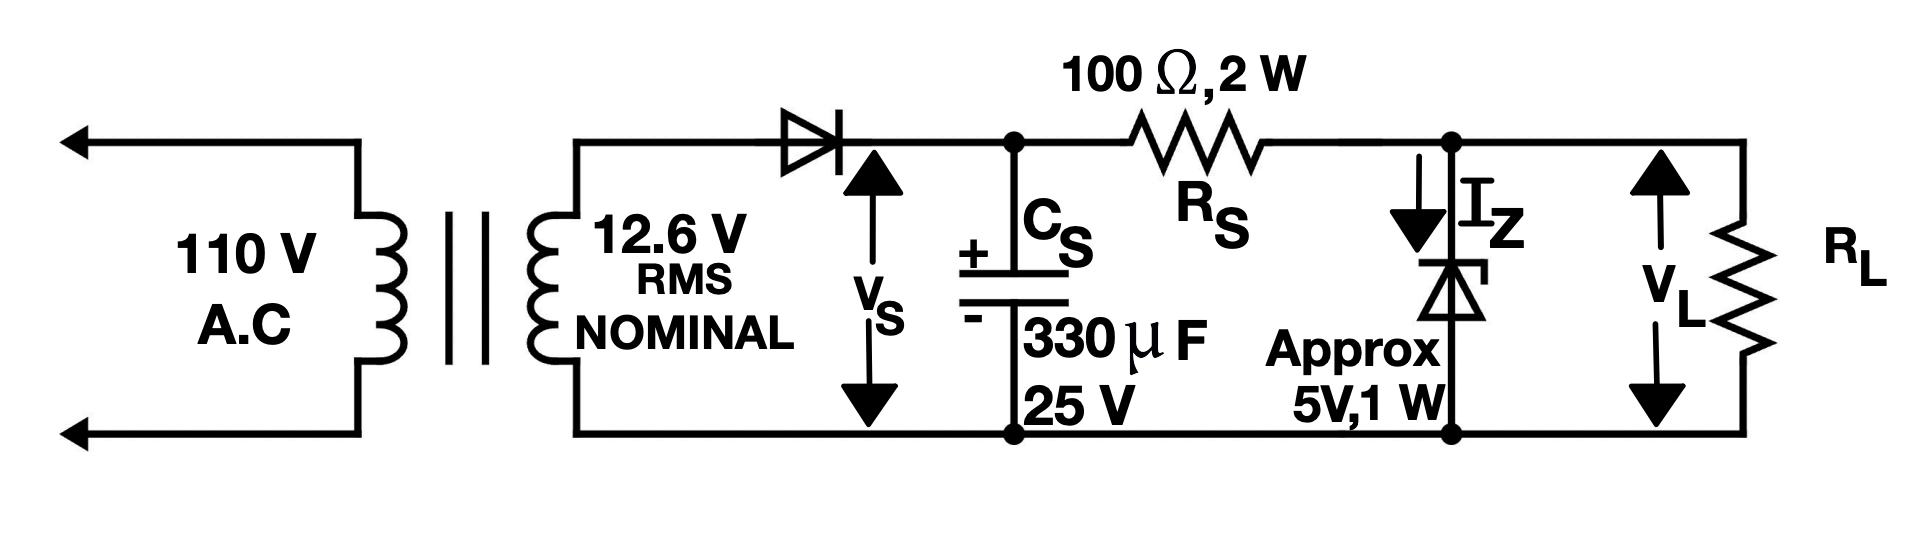
\includegraphics[width=\textwidth]{figures/F/schematic.png}
		\caption{Schematic for experiment F \\ \protect\cite{labManual}}
	\end{minipage}
\end{figure}
\subsubsection{Part 1}\label{method::F1}
The adjustable transformer was adjusted to achieve the correct transformer voltage. This was verified with the oscilloscope. Then the oscilloscope was set up to measure $V_S$ on channel 1 and $V_L$ on channel two. AC and DC RMS voltage values were recorded, and the data was saved to a USB flash drive. This procedure was repeated for transformer input voltages of $9.7\unit{\volt}_{\rm rms}$, $12.6\unit{\volt}_{\rm rms}$ and $14.9\unit{\volt}_{\rm rms}$. For these experiments, $R_L$ was set to $100\Omega$.
\subsubsection{Part 2}\label{method::F2}
In the second part of this experiment, the transformer was reset to $12.6\unit{\volt}_{\rm rms}$ using the oscilloscope again for verification. A multimeter was also connected to measure the value of $I_L$ between the output of the zener diode and the top side of the resistor. $V_S$ was connected to channel 1 and $V_L$ was connected to channel 2. Both DC and AC RMS voltages were recorded as well as the multimeter readout for $I_L$. The data was then exported onto a USB flash drive. This was repeated for $R_L$ resistor values of $56\Omega$, $100\Omega$ and $2.7\unit{k\ohm}$.

\subsection{Results and Analysis}
\subsubsection{Part 1}
\begin{figure}[H]    \centering    \begin{tabular}{|l|c|c|}
        \hline
        Measured Value & AC RMS & DC RMS \\
        \hline
        $V_{L} - 12.6\unit{V}$ & $40\pm 10\unit{mV}$ & $4.99\pm 0.01\unit{V}$ \\
        $V_{L} - 14.9\unit{V}$ & $30\pm 10\unit{mV}$ & $5.06\pm 0.01\unit{V}$ \\
        $V_{L} - 9.7\unit{V}$ & $130\pm 10\unit{mV}$ & $4.75\pm 0.01\unit{V}$ \\
        $V_{S} - 12.6\unit{V}$ & $850\pm 10\unit{mV}$ & $13.10\pm 0.01\unit{V}$ \\
        $V_{S} - 14.9\unit{V}$ & $1.08\pm 0.01\unit{V}$ & $15.30\pm 0.01\unit{V}$ \\
        $V_{S} - 9.7\unit{V}$ & $580\pm 10\unit{mV}$ & $10.13\pm 0.01\unit{V}$ \\
        \hline
    \end{tabular}    \caption{Oscilloscope measured voltages for experiment F Part 1}\end{figure}
$9.7\unit{V}$:  $RF=0.027\pm 0.002$\\
$12.6\unit{V}$: $RF=0.008\pm 0.002\unit{V}$\\
$14.9\unit{V}$: $RF=0.005\pm 0.002\unit{V}$\\

These relatively low ripple factors are reflected in the $V_L$ plots of each of these circuits in \bref{data::F}{Figure 47}, \bref{data::F}{Figure 49} and \bref{data::F}{Figure 51}. All of these plots have a very low waveform amplitude. However. in the $9.7\unit{V}$ experiment, the amplitude of the waveform is noticeably higher. This suggests that the lower voltage does not allow the Zener diode to maintain its reference voltage as well.
\subsubsection{Part 2}
\begin{figure}[H]    \centering    \begin{tabular}{|l|c|c|}
        \hline
        Measured Value & AC RMS & DC RMS \\
        \hline
        $V_{L} - 2.7\unit{k\ohm}$ & $40\pm 10\unit{mV}$ & $5.01\pm 0.01\unit{V}$ \\
        $V_{L} - 560\unit{\ohm}$ & $30\pm 10\unit{mV}$ & $5.09\pm 0.01\unit{V}$ \\
        $V_{L} - 56\unit{\ohm}$ & $230\pm 10\unit{mV}$ & $4.51\pm 0.01\unit{V}$ \\
        $V_{S} - 2.7\unit{k\ohm}$ & $840\pm 10\unit{mV}$ & $13.00\pm 0.01\unit{V}$ \\
        $V_{S} - 560\unit{\ohm}$ & $830\pm 10\unit{mV}$ & $13.00\pm 0.01\unit{V}$ \\
        $V_{S} - 56\unit{\ohm}$ & $860\pm 10\unit{mV}$ & $12.72\pm 0.01\unit{V}$ \\
        \hline
    \end{tabular}    \caption{Oscilloscope measured voltages for experiment F Part 2}\end{figure}
For the $56\unit{\ohm}$ $R_L$ value, the ripple factor was $0.005\pm0.002$\\
For the $560\unit{\ohm}$ $R_L$ value, the ripple factor was $0.001\pm0.002$\\
For the $2.7\unit{k\ohm}$ $R_L$ value, the ripple factor was $0.001\pm0.002$\\\\
The fact that the second and third ripple factors are so much lower is similar to the first part. Both parts of \bref{exp::F}{Experiment F} suggest that the Zener diode provides a very stable signal past a specific resistance load and transformer voltage. The ripple factors are all very near zero and this is clearly reflected in the oscilloscope plots of figures \bref{data::F4}{Figure 53} $\rightarrow$ \bref{data::F6}{Figure 58}



\section{Experiment G}\label{exp::G}
\subsection{Methodology}\label{method::G}
In this experiment, the zener diode, transistor regulation circuit depicted in \bref{apparatus::G}{Figure 16} was assembled.
\begin{figure}[H]\label{apparatus::G}
	\centering
	\begin{minipage}[c]{0.45\textwidth}
		\centering
		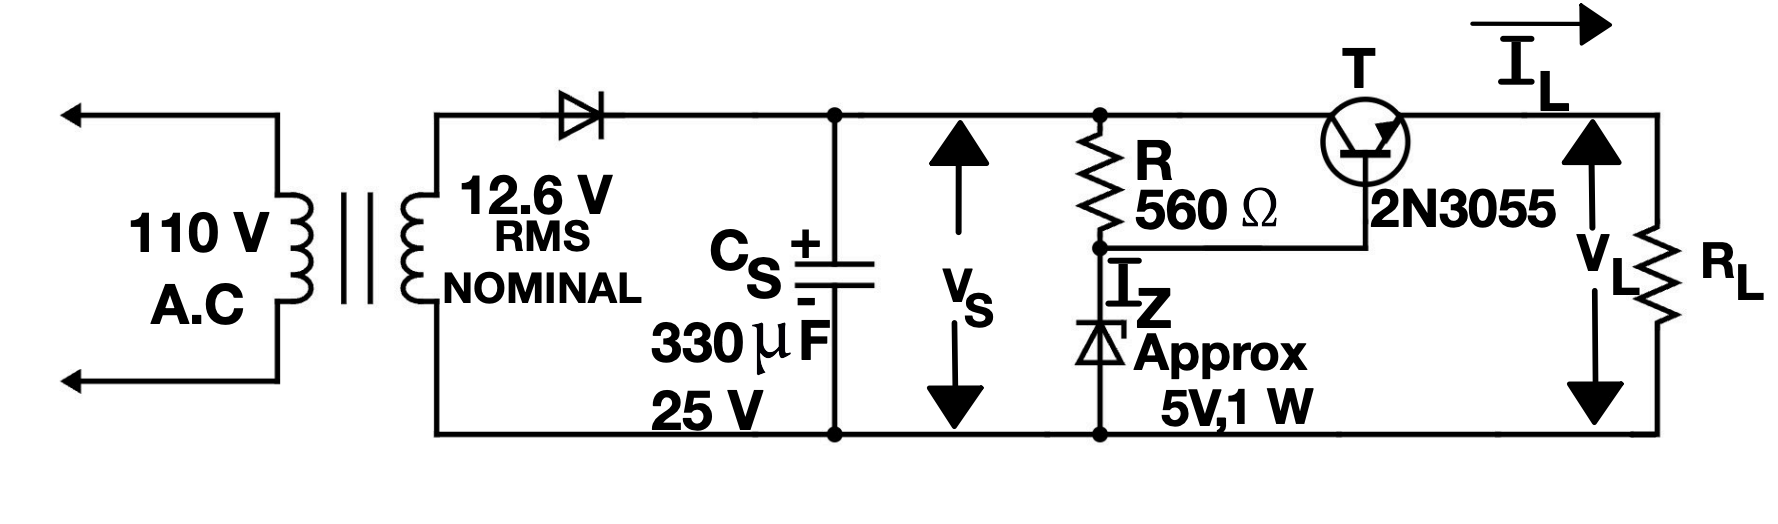
\includegraphics[width=\textwidth]{figures/G/schematic.png}
		\caption{Schematic for experiment G \\ \protect\cite{labManual}}
	\end{minipage}
\end{figure}
\subsubsection{Part 1}\label{method::G1}
The adjustable transformer was adjusted to the appropriate voltage. This was verified with an oscilloscope measurement over the terminals of the transformer. $R_L$ was set up to be a $100\Omega$ resistor. $V_L$ was connected to channel 1 and $V_S$ was connected to channel 2. A multimeter was set up between the transistor and load to measure the value of $I_L$. DC and AC RMS voltage measurements were made and the data was saved onto a USB flash drive. This was repeated for transformer voltages of $9.7\unit{\volt}_{\rm rms}$, $12.6\unit{\volt}_{\rm rms}$ and $14.9\unit{\volt}_{\rm rms}$.
\subsubsection{Part 2}\label{method::G2}
The voltage was then reset to $12.6\unit{\volt}_{\rm rms}$, verified with the oscilloscope. With constant voltage, the same measurements were then taken on the system, with $R_L$ values of $56\Omega$ and $2.7\unit{k\volt}$.
\subsection{Results and Analysis}
\subsubsection{Part 1}
\begin{figure}[H]    \centering    \begin{tabular}{|l|c|c|}
        \hline
        Measured Value & AC RMS & DC RMS \\
        \hline
        $V_{L} - 12.6\unit{V}$ & $20\pm 10\unit{mV}$ & $4.35\pm 0.01\unit{V}$ \\
        $V_{L} - 14.9\unit{V}$ & $20\pm 10\unit{mV}$ & $4.39\pm 0.01\unit{V}$ \\
        $V_{L} - 9.7\unit{V}$ & $30\pm 10\unit{mV}$ & $4.23\pm 0.01\unit{V}$ \\
        $V_{S} - 12.6\unit{V}$ & $810\pm 10\unit{mV}$ & $13.70\pm 0.01\unit{V}$ \\
        $V_{S} - 14.9\unit{V}$ & $890\pm 10\unit{mV}$ & $16.60\pm 0.01\unit{V}$ \\
        $V_{S} - 9.7\unit{V}$ & $710\pm 10\unit{mV}$ & $10.16\pm 0.01\unit{V}$ \\
        \hline
    \end{tabular}    \caption{Oscilloscope measured voltages for experiment G Part 1}\end{figure}
For the $9.7\unit{V}$ input voltage, the ripple factor was $0.001\pm 0.002\unit{V}$\\
For the $12.6\unit{V}$ input voltage, the ripple factor was $0.001\pm 0.002\unit{V}$\\
For the $14.9\unit{V}$ input voltage, the ripple factor was $0\pm 0.002\unit{V}$\\\\
The similarity of these values through each of the input voltage values compared to the same values in \bref{exp::F}{Experiment F}, suggest that the Zener diode/transistor system provides a system that is less affected by fluctuations in the input voltage.
\subsubsection{Part 2}
\begin{figure}[H]    \centering    \begin{tabular}{|l|c|c|}
        \hline
        Measured Value & AC RMS & DC RMS \\
        \hline
        $V_{L} - 2.7\unit{k\ohm}$ & $20\pm 10\unit{mV}$ & $4.21\pm 0.01\unit{V}$ \\
        $V_{L} - 56\unit{\ohm}$ & $30\pm 10\unit{mV}$ & $3.56\pm 0.01\unit{V}$ \\
        $V_{S} - 2.7\unit{k\ohm}$ & $480\pm 10\unit{mV}$ & $15.30\pm 0.01\unit{V}$ \\
        $V_{S} - 56\unit{\ohm}$ & $1.03\pm 0.01\unit{V}$ & $12.80\pm 0.01\unit{V}$ \\
        \hline
    \end{tabular}    \caption{Oscilloscope measured voltages for experiment G Part 2}\end{figure}
For the $56\unit{\ohm}$ $R_L$ value, the ripple factor was $0.001\pm0.003$\\
For the $2.7\unit{k\ohm}$ $R_L$ value, the ripple factor was $0\pm 0.002\unit{V}$\\\\
Considering that we were unable to get an adequate third sample, it is hard to specify a specific trend in the data for this section. However, throughout both parts of this experiment, the ripple factor has been the lowest achieved by any of the circuits that were tested. This approach does only use half-wave rectification, therefore it is possible that if a similar strategy could be applied to a full wave or bridge rectification system this might yield even better results.




\section{Experiment H}\label{exp::H}
\subsection{Methodology}\label{method::H}
For this experiment, we assembled the voltage doubler rectifier shown in \bref{apparatus::H}{Figure 15}. The assembled apparatus is shown in \bref{apparatus::H}{Figure 16}.
\begin{figure}[H]\label{apparatus::H}
	\centering
	\begin{minipage}[c]{0.45\textwidth}
		\centering
		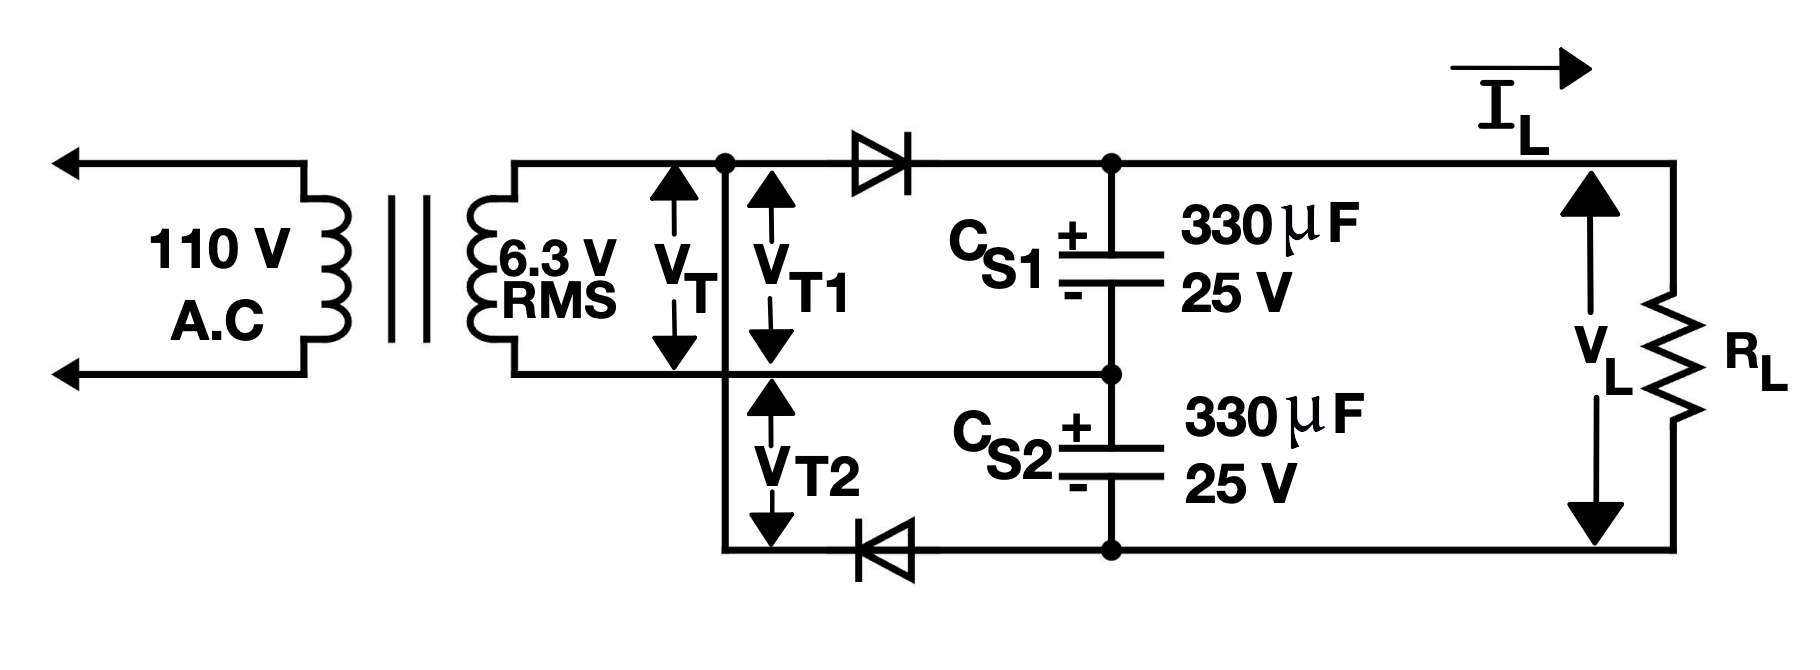
\includegraphics[width=\textwidth]{figures/H/schematic.png}
		\caption{Schematic for experiment H \\ \protect\cite{labManual}}
	\end{minipage}
\end{figure}
For each of the values $V_T$, $V_{T1}$, $V_{T2}$ and $V_L$, the oscilloscope was set to measure one of these values on channel 1. The AC and DC RMS voltages were noted, and the oscilloscope data was saved onto a USB flash drive. This was repeated for $R_L$ values of $270\unit{\ohm}$, $1\unit{k\ohm}$ and $2.7\unit{k\ohm}$



\subsection{Results and Analysis}
Voltage values for $R_L = 270\unit{\ohm}$\\
\begin{figure}[H]    \centering    \begin{tabular}{|l|c|c|}
        \hline
        Measured Value & AC RMS & DC RMS \\
        \hline
        $V_{L}$ & $530\pm 10\unit{mV}$ & $13.60\pm 0.01\unit{V}$ \\
        $V_{T1}$ & $6.20\pm 0.01\unit{V}$ & $6.20\pm 0.01\unit{V}$ \\
        $V_{T2}$ & $6.21\pm 0.01\unit{V}$ & $6.21\pm 0.01\unit{V}$ \\
        $V_{T}$ & $6.21\pm 0.01\unit{V}$ & $6.21\pm 0.01\unit{V}$ \\
        \hline
    \end{tabular}    \caption{Oscilloscope measured voltages for experiment H Part 1}\end{figure}
Voltage values for $R_L = 1\unit{k\ohm}$\\
\begin{figure}[H]    \centering    \begin{tabular}{|l|c|c|}
        \hline
        Measured Value & AC RMS & DC RMS \\
        \hline
        $V_{L}$ & $190\pm 10\unit{mV}$ & $15.80\pm 0.01\unit{V}$ \\
        $V_{T1}$ & $6.59\pm 0.01\unit{V}$ & $6.59\pm 0.01\unit{V}$ \\
        $V_{T2}$ & $6.58\pm 0.01\unit{V}$ & $6.58\pm 0.01\unit{V}$ \\
        $V_{T}$ & $6.59\pm 0.01\unit{V}$ & $6.59\pm 0.01\unit{V}$ \\
        \hline
    \end{tabular}    \caption{Oscilloscope measured voltages for experiment H Part 2}\end{figure}
Voltage values for $R_L = 2.7\unit{k\ohm}$\\
\begin{figure}[H]    \centering    \begin{tabular}{|l|c|c|}
        \hline
        Measured Value & AC RMS & DC RMS \\
        \hline
        $V_{L}$ & $80\pm 10\unit{mV}$ & $16.70\pm 0.01\unit{V}$ \\
        $V_{T1}$ & $6.70\pm 0.01\unit{V}$ & $6.70\pm 0.01\unit{V}$ \\
        $V_{T2}$ & $6.71\pm 0.01\unit{V}$ & $6.71\pm 0.01\unit{V}$ \\
        $V_{T}$ & $6.70\pm 0.01\unit{V}$ & $6.70\pm 0.01\unit{V}$ \\
        \hline
    \end{tabular}    \caption{Oscilloscope measured voltages for experiment H Part 3}\end{figure}

This particular circuit works by charging capacitors in cycles of the AC power and then discharging them in series, to the load resulting in an output voltage. In comparison to the full wave rectifier shown in \bref{apparatus::B}{Figure 3} the diodes used in the voltage doubler need to handle peak inverse voltages because they block an amount of output during off cycles. The inverse voltages will be much higher in this circuit due to the capacitors.

\section{Conclusion}
In this lab, we compared various AC to DC conversion methods. First comparing rectifiers, we determined that the best rectification method in terms of \bref{eqn::ripple}{Ripple factor} was the bridge rectifier in \bref{method::C}{Experiment C}. The best signal that we achieved by the same metric was the zener diode transistor regulation circuit with half-wave rectification. A future study could look into the feasibility of combining a more effective rectification method such as the bridge rectifier with higher quality smoothing such as the zener diode transitor circuit. This could potentially provide a better quality DC signal. One major limitation of this lab report was the focus primarily on the ripple factor, leaving out the efficiency of each circuit in terms of power loss. This is a key aspect of the conversion that causes a substantial trade-off in real life scenarios. Taking appropriate measurements to calculate the power loss for every circuit would provide a more comprehensive overview of their effectiveness.
\newpage\appendix
\section{Sample calculation for ripple and error propagation}\label{appdx::A}
In \bref{method::A}{Experiment A}, the $V_L$ measurement had a ACRMS value of $3.64\pm 0.01V$ and a DCRMS value of $4.61\pm0.01V$. The \bref{eqn::ripple}{Ripple Factor} was calculated as follows:
\begin{align*}
	RF = {3.64\over 4.61} =  0.790
\end{align*}
The error was propagated using \bref{prop::div}{Division Propagation} as follows:
\begin{align*}
	\Delta (3.64/4.61) = \sqrt{ \left({0.01\over 3.64}\right) + \left({0.01\over 4.61}\right)}= 0.004
\end{align*}
This gives the final value of $0.790 \pm 0.004$
\section{Oscilloscope screens}
\subsection{Experiment A}
\begin{figure}[H]\label{data::A}
	\centering
	\begin{minipage}[c]{0.45\textwidth}
		\centering
		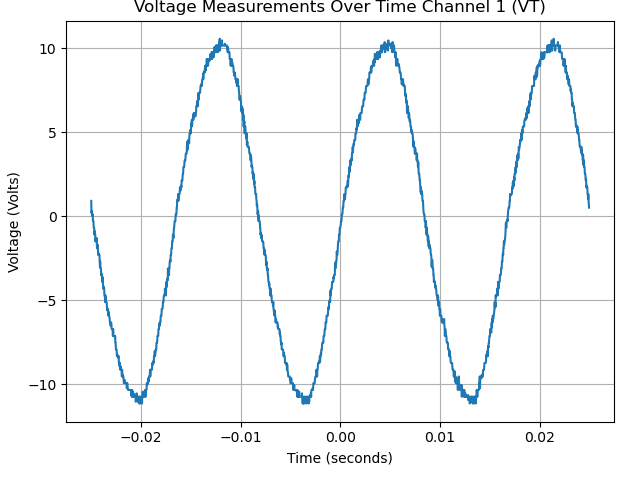
\includegraphics[width=\textwidth]{figures/A/1--ch1.png}
		\caption{$V_T$ oscilloscope readout for \bref{exp::A}{Experiment A}}
	\end{minipage}
	\hfill
	\begin{minipage}[c]{0.45\textwidth}
		\centering
		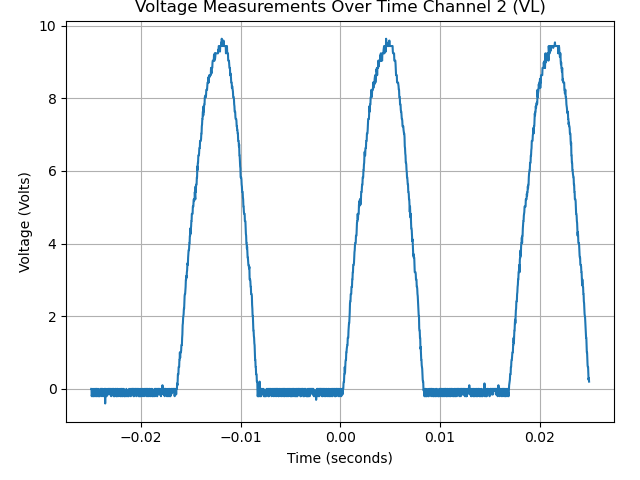
\includegraphics[width=\textwidth]{figures/A/1--ch2.png}
		\caption{$V_L$ oscilloscope readout for \bref{exp::A}{Experiment A}}
	\end{minipage}
\end{figure}

\subsection{Experiment B}

\begin{figure}[H]\label{data::B}
	\centering
	\begin{minipage}[c]{0.45\textwidth}
		\centering
		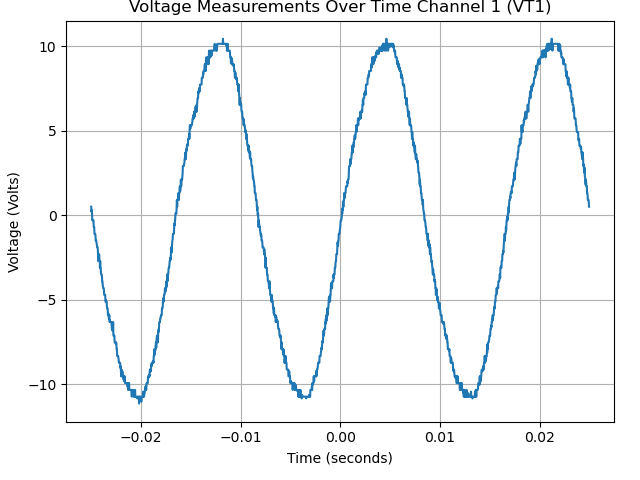
\includegraphics[width=\textwidth]{figures/B/1--ch1.png}
		\caption{$V_{T1}$ oscilloscope readout for \bref{exp::B}{Experiment B}}
	\end{minipage}
	\hfill
	\begin{minipage}[c]{0.45\textwidth}
		\centering
		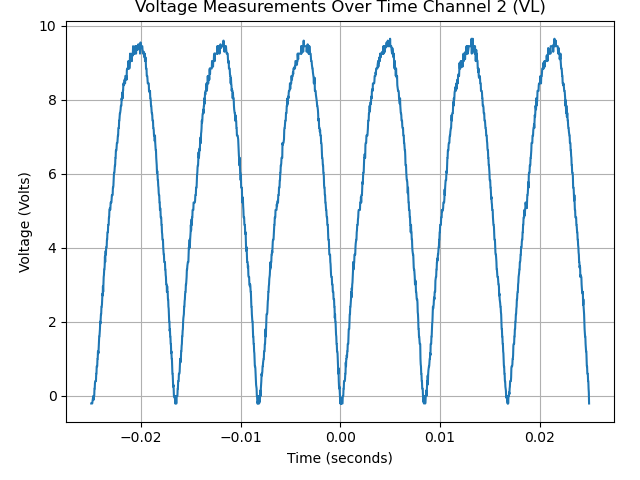
\includegraphics[width=\textwidth]{figures/B/1--ch2.png}
		\caption{$V_{L}$ oscilloscope readout for \bref{exp::B}{Experiment B}}
	\end{minipage}
\end{figure}

\begin{figure}[H]\label{data::B2}
	\centering
	\begin{minipage}[c]{0.45\textwidth}
		\centering
		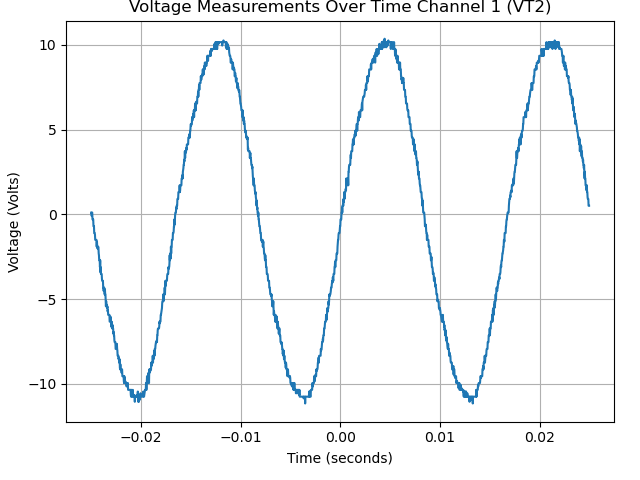
\includegraphics[width=\textwidth]{figures/B/2--ch1.png}
		\caption{$V_{T2}$ oscilloscope readout for \bref{exp::B}{Experiment B}}
	\end{minipage}
	\hfill
	\begin{minipage}[c]{0.45\textwidth}
		\centering
		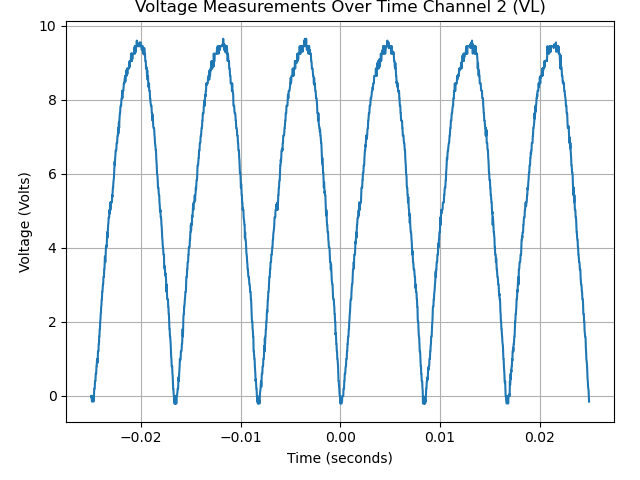
\includegraphics[width=\textwidth]{figures/B/2--ch2.png}
		\caption{$V_{L}$ oscilloscope readout for \bref{exp::B}{Experiment B}}
	\end{minipage}
\end{figure}
\subsection{Experiment C}
\begin{figure}[H]\label{data::C}
	\centering
	\begin{minipage}[c]{0.45\textwidth}
		\centering
		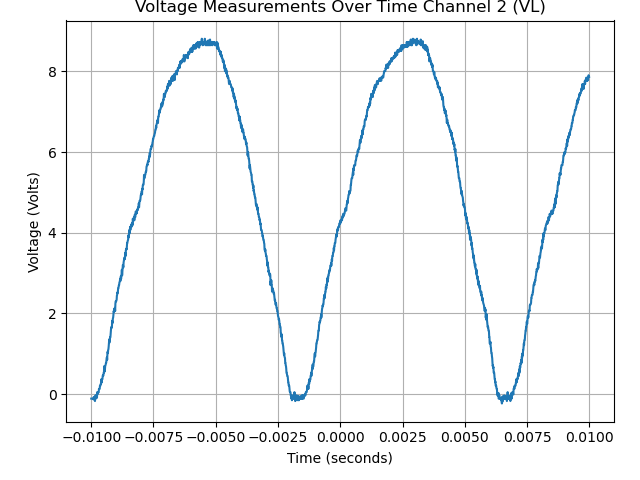
\includegraphics[width=\textwidth]{figures/C/1--ch2.png}
		\caption{$V_{L}$ oscilloscope readout for \bref{exp::C}{Experiment C}}
	\end{minipage}
	\hfill
	\begin{minipage}[c]{0.45\textwidth}
		\centering
		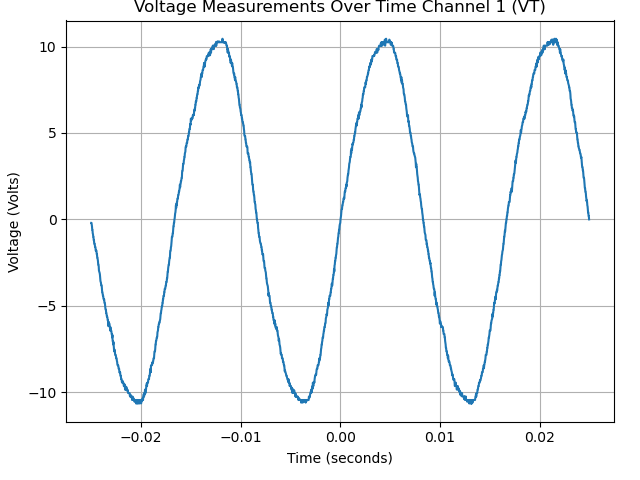
\includegraphics[width=\textwidth]{figures/C/2--ch1.png}
		\caption{$V_{L}$ oscilloscope readout for \bref{exp::C}{Experiment C}}
	\end{minipage}
\end{figure}

\subsection{Experiment D}
\subsubsection{Part 1}
\begin{figure}[H]\label{data::D}
	\centering
	\begin{minipage}[c]{0.45\textwidth}
		\centering
		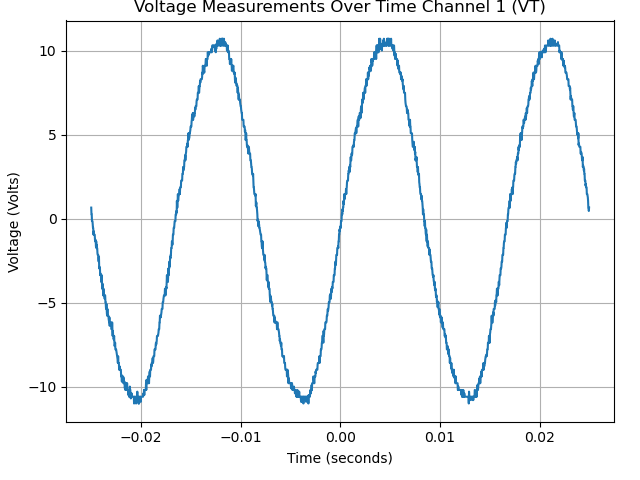
\includegraphics[width=\textwidth]{figures/D/1--ch1.png}
	    \caption{$V_{T}$ oscilloscope readout for \bref{exp::D}{Experiment D} $2.7\unit{k\ohm}$ resistor}
	\end{minipage}
	\hfill
	\begin{minipage}[c]{0.45\textwidth}
		\centering
		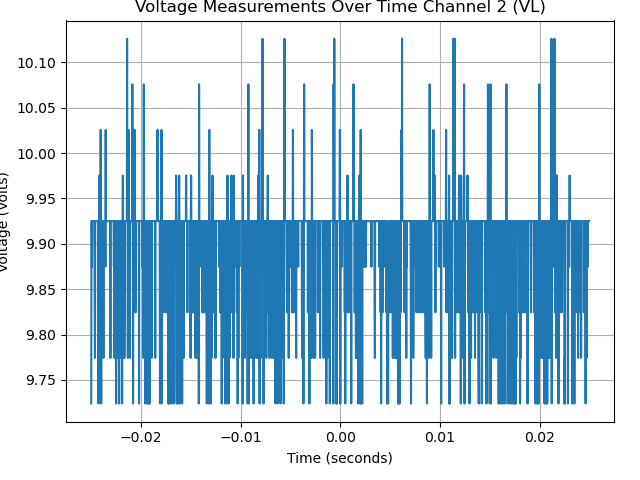
\includegraphics[width=\textwidth]{figures/D/1--ch2.png}
	    \caption{$V_{L}$ oscilloscope readout for \bref{exp::D}{Experiment D} $2.7\unit{k\ohm}$ resistor}
	\end{minipage}
\end{figure}
\begin{figure}[H]\label{data::D2}
	\centering
	\begin{minipage}[c]{0.45\textwidth}
		\centering
		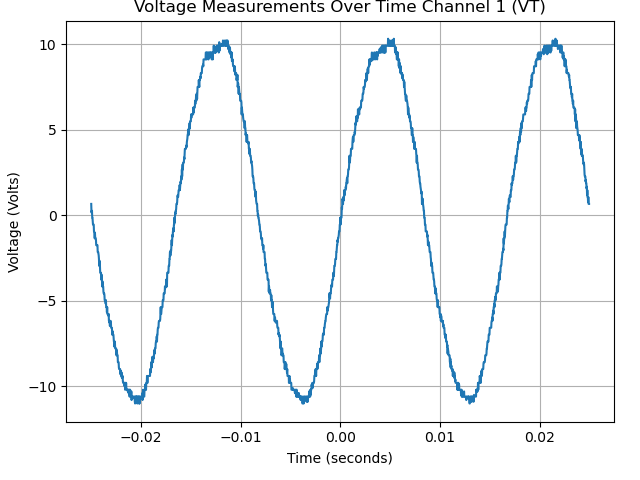
\includegraphics[width=\textwidth]{figures/D/2--ch1.png}
	    \caption{$V_{T}$ oscilloscope readout for \bref{exp::D}{Experiment D} $560\unit{\ohm}$ resistor}
	\end{minipage}
	\hfill
	\begin{minipage}[c]{0.45\textwidth}
		\centering
		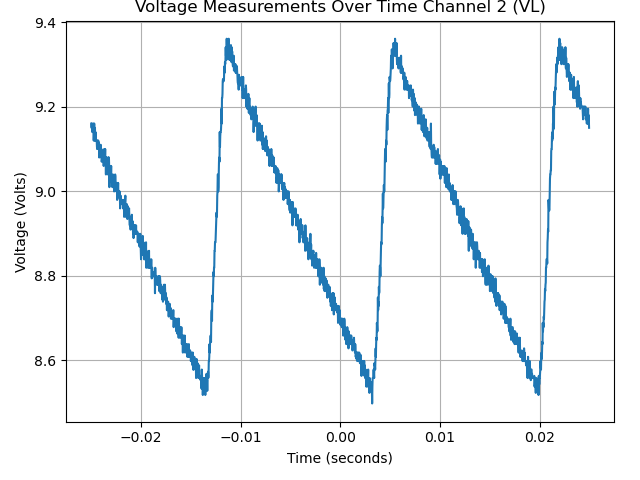
\includegraphics[width=\textwidth]{figures/D/2--ch2.png}
	    \caption{$V_{L}$ oscilloscope readout for \bref{exp::D}{Experiment D} $560\unit{\ohm}$ resistor}
	\end{minipage}
\end{figure}
\begin{figure}[H]\label{data::D3}
	\centering
	\begin{minipage}[c]{0.45\textwidth}
		\centering
		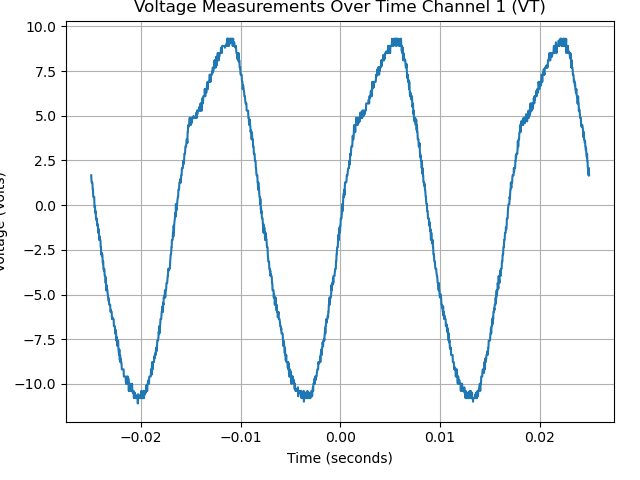
\includegraphics[width=\textwidth]{figures/D/3--ch1.png}
	    \caption{$V_{T}$ oscilloscope readout for \bref{exp::D}{Experiment D} $56\unit{\ohm}$ resistor}
	\end{minipage}
	\hfill
	\begin{minipage}[c]{0.45\textwidth}
		\centering
		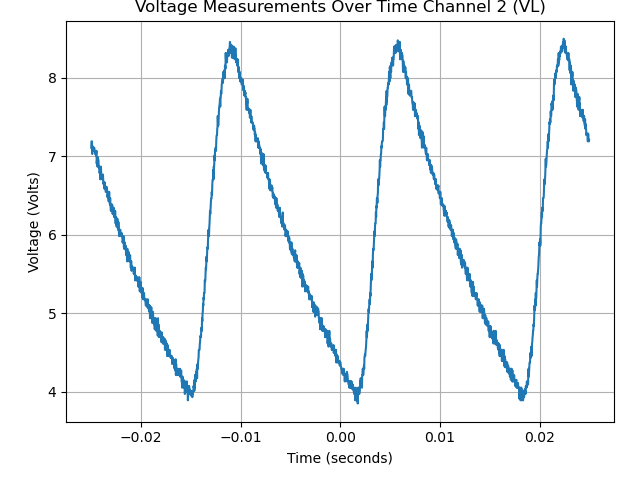
\includegraphics[width=\textwidth]{figures/D/3--ch2.png}
	    \caption{$V_{L}$ oscilloscope readout for \bref{exp::D}{Experiment D} $56\unit{\ohm}$ resistor}
	\end{minipage}
\end{figure}
\subsubsection{Part 2}
\begin{figure}[H]\label{data::D4}
	\centering
	\begin{minipage}[c]{0.45\textwidth}
		\centering
		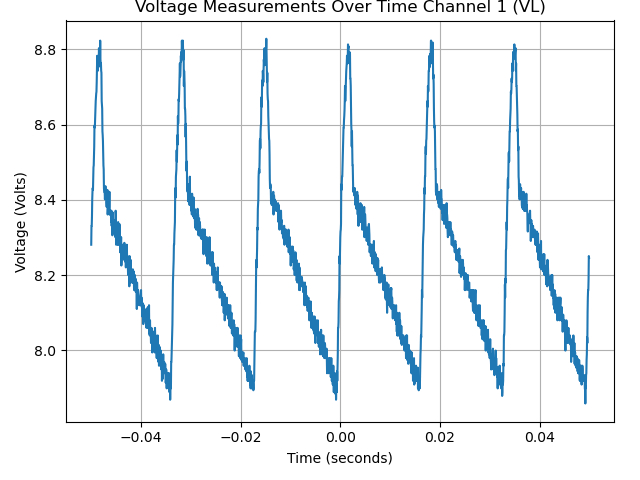
\includegraphics[width=\textwidth]{figures/D/4--ch1.png}
	    \caption{$V_{L}$ oscilloscope readout for \bref{exp::D}{Experiment D} part 2 $560\unit{\ohm}$ resistor}
	\end{minipage}
	\hfill
	\begin{minipage}[c]{0.45\textwidth}
		\centering
		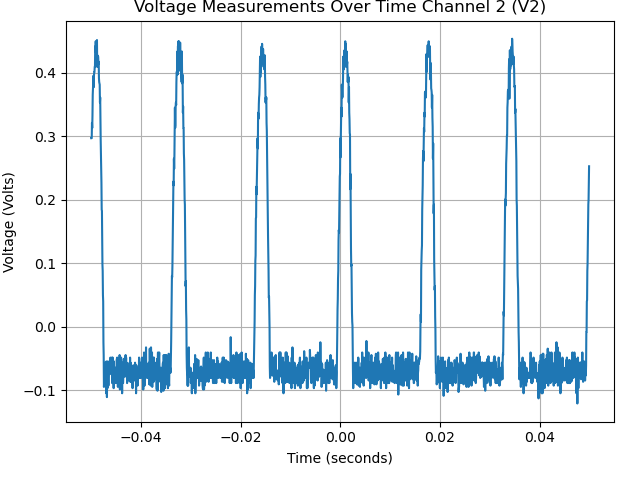
\includegraphics[width=\textwidth]{figures/D/4--ch2.png}
	    \caption{$V_{2}$ oscilloscope readout for \bref{exp::D}{Experiment D} part 2 $560\unit{\ohm}$ resistor}
	\end{minipage}
\end{figure}
\begin{figure}[H]\label{data::D5}
	\centering
	\begin{minipage}[c]{0.45\textwidth}
		\centering
		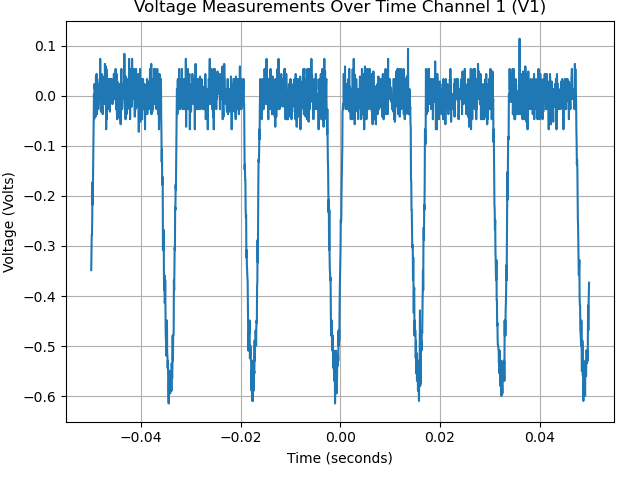
\includegraphics[width=\textwidth]{figures/D/5--ch1.png}
	    \caption{$V_{1}$ oscilloscope readout for \bref{exp::D}{Experiment D} part 2 $560\unit{\ohm}$ resistor}
	\end{minipage}
	\hfill
	\begin{minipage}[c]{0.45\textwidth}
		\centering
		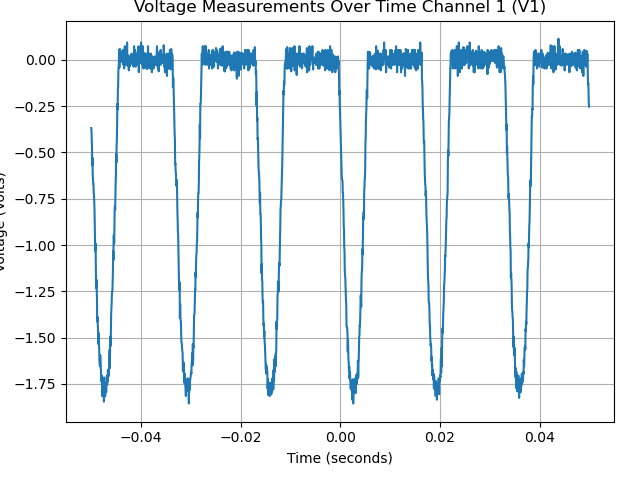
\includegraphics[width=\textwidth]{figures/D/6--ch1.png}
	    \caption{$V_{1}$ oscilloscope readout for \bref{exp::D}{Experiment D} part 2 $56\unit{\ohm}$ resistor}
	\end{minipage}
\end{figure}
\begin{figure}[H]\label{data::D6}
	\centering
	\begin{minipage}[c]{0.45\textwidth}
		\centering
		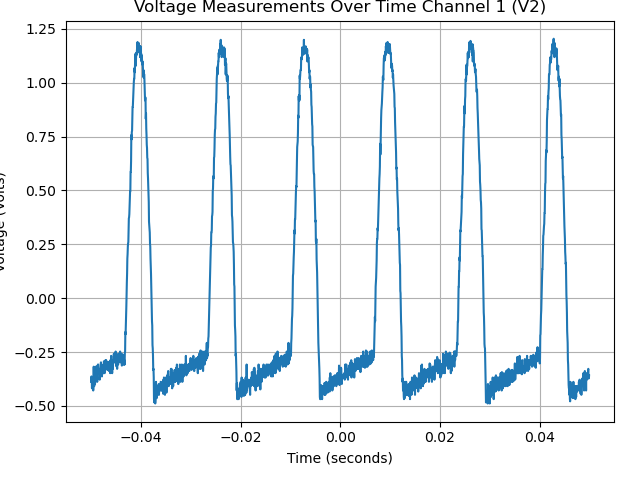
\includegraphics[width=\textwidth]{figures/D/7--ch1.png}
	    \caption{$V_{2}$ oscilloscope readout for \bref{exp::D}{Experiment D} part 2 $56\unit{\ohm}$ resistor}
	\end{minipage}
	\hfill
	\begin{minipage}[c]{0.45\textwidth}
		\centering
		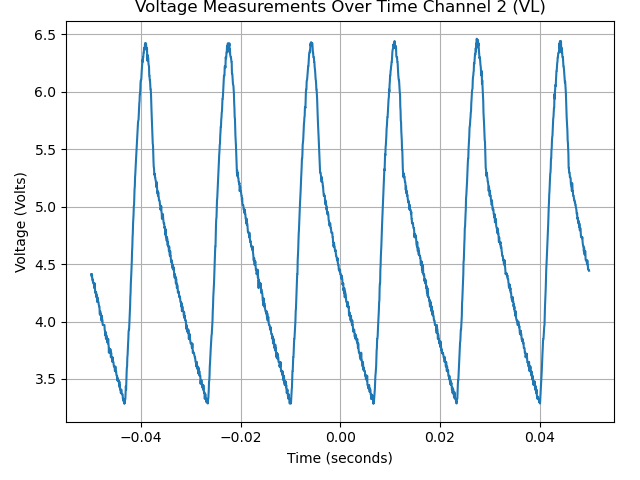
\includegraphics[width=\textwidth]{figures/D/7--ch2.png}
	    \caption{$V_{L}$ oscilloscope readout for \bref{exp::D}{Experiment D} part 2 $56\unit{\ohm}$ resistor}
	\end{minipage}
\end{figure}
\subsection{Experiment E}
\begin{figure}[H]\label{data::E}
	\centering
	\begin{minipage}[c]{0.45\textwidth}
		\centering
		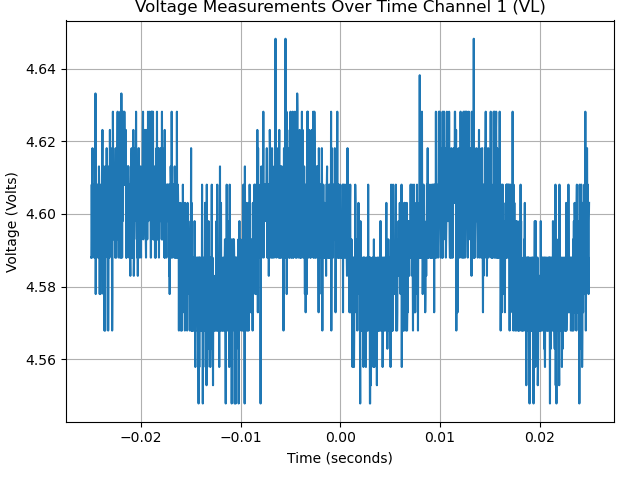
\includegraphics[width=\textwidth]{figures/E/1--ch1.png}
	    \caption{$V_{L}$ oscilloscope readout for \bref{exp::E}{Experiment E} (DC coupling)}
	\end{minipage}
	\hfill
	\begin{minipage}[c]{0.45\textwidth}
		\centering
		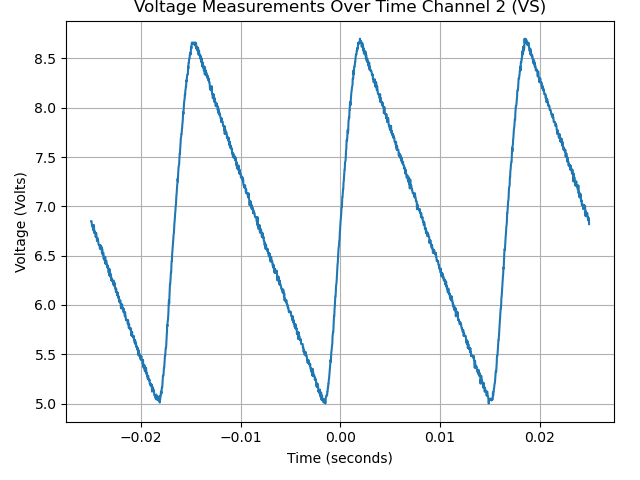
\includegraphics[width=\textwidth]{figures/E/1--ch2.png}
	    \caption{$V_{S}$ oscilloscope readout for \bref{exp::E}{Experiment E} (DC coupling)}
	\end{minipage}
\end{figure}
\begin{figure}[H]\label{data::E2}
	\centering
	\begin{minipage}[c]{0.45\textwidth}
		\centering
		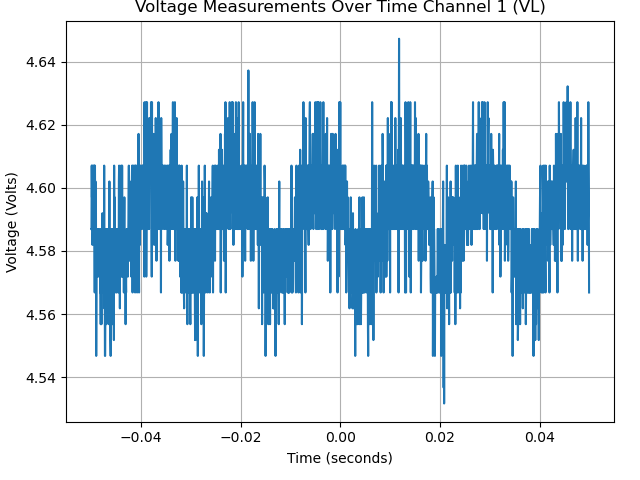
\includegraphics[width=\textwidth]{figures/E/2--ch1.png}
	    \caption{$V_{L}$ oscilloscope readout for \bref{exp::E}{Experiment E} (AC coupling)}
	\end{minipage}
	\hfill
	\begin{minipage}[c]{0.45\textwidth}
		\centering
		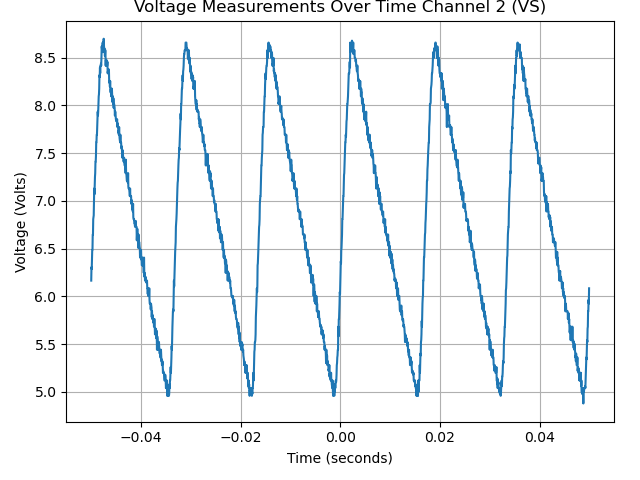
\includegraphics[width=\textwidth]{figures/E/2--ch2.png}
	    \caption{$V_{S}$ oscilloscope readout for \bref{exp::E}{Experiment E} (AC coupling)}
	\end{minipage}
\end{figure}
\subsection{Experiment F}
\begin{figure}[H]\label{data::F}
	\centering
	\begin{minipage}[c]{0.45\textwidth}
		\centering
		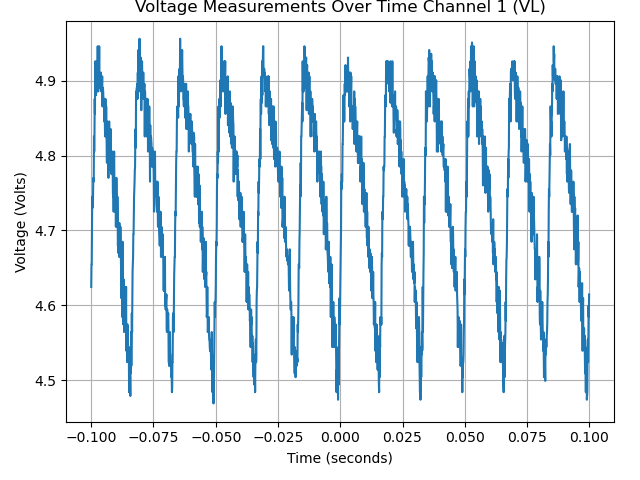
\includegraphics[width=\textwidth]{figures/F/1--ch1.png}
	    \caption{$V_{L}$ oscilloscope readout for \bref{exp::F}{Experiment F} $9.7\unit V$ }
	\end{minipage}
	\hfill
	\begin{minipage}[c]{0.45\textwidth}
		\centering
		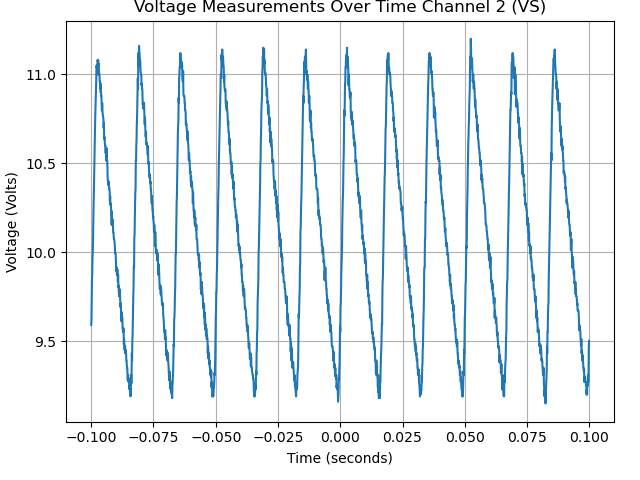
\includegraphics[width=\textwidth]{figures/F/1--ch2.png}
	    \caption{$V_{S}$ oscilloscope readout for \bref{exp::F}{Experiment F} $9.7\unit V$ }
	\end{minipage}
\end{figure}
\begin{figure}[H]\label{data::F2}
	\centering
	\begin{minipage}[c]{0.45\textwidth}
		\centering
		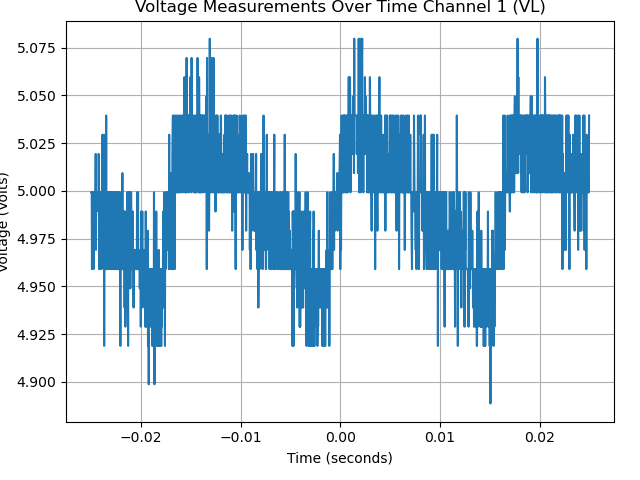
\includegraphics[width=\textwidth]{figures/F/2--ch1.png}
	    \caption{$V_{L}$ oscilloscope readout for \bref{exp::F}{Experiment F} $12.6\unit V$ }
	\end{minipage}
	\hfill
	\begin{minipage}[c]{0.45\textwidth}
		\centering
		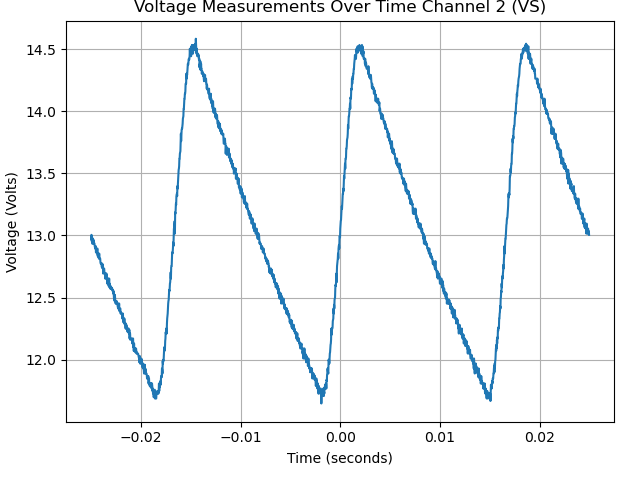
\includegraphics[width=\textwidth]{figures/F/2--ch2.png}
	    \caption{$V_{S}$ oscilloscope readout for \bref{exp::F}{Experiment F} $12.6\unit V$ }
	\end{minipage}
\end{figure}
\begin{figure}[H]\label{data::F3}
	\centering
	\begin{minipage}[c]{0.45\textwidth}
		\centering
		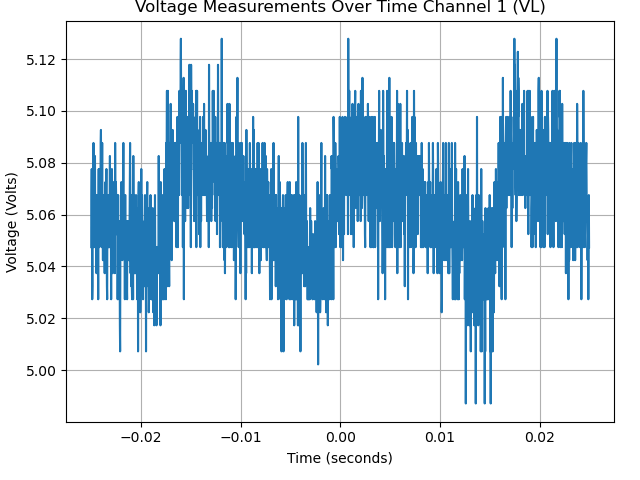
\includegraphics[width=\textwidth]{figures/F/3--ch1.png}
	    \caption{$V_{L}$ oscilloscope readout for \bref{exp::F}{Experiment F} $14.9\unit V$ }
	\end{minipage}
	\hfill
	\begin{minipage}[c]{0.45\textwidth}
		\centering
		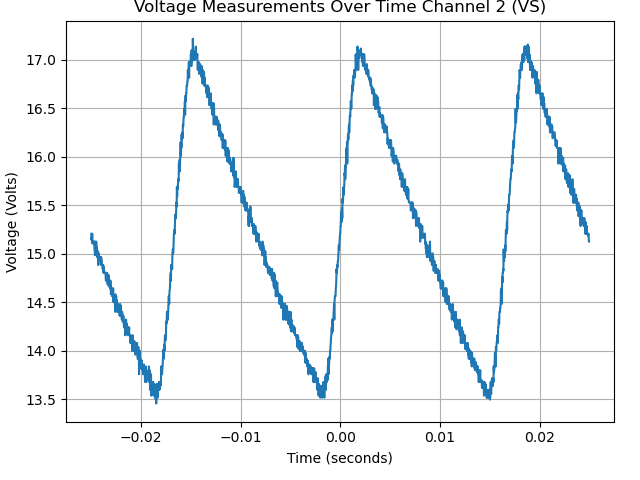
\includegraphics[width=\textwidth]{figures/F/3--ch2.png}
	    \caption{$V_{S}$ oscilloscope readout for \bref{exp::F}{Experiment F} $14.9\unit V$ }
	\end{minipage}
\end{figure}
\begin{figure}[H]\label{data::F4}
	\centering
	\begin{minipage}[c]{0.45\textwidth}
		\centering
		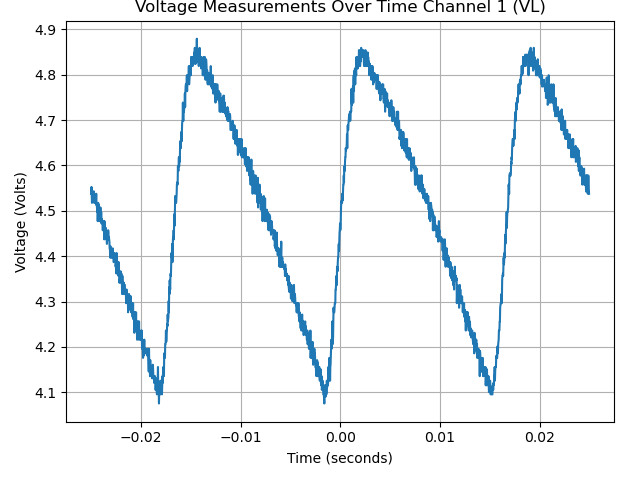
\includegraphics[width=\textwidth]{figures/F/4--ch1.png}
	    \caption{$V_L$ oscilloscope readout for \bref{exp::F}{Experiment F} $56\unit{\ohm}$ }
	\end{minipage}
	\hfill
	\begin{minipage}[c]{0.45\textwidth}
		\centering
		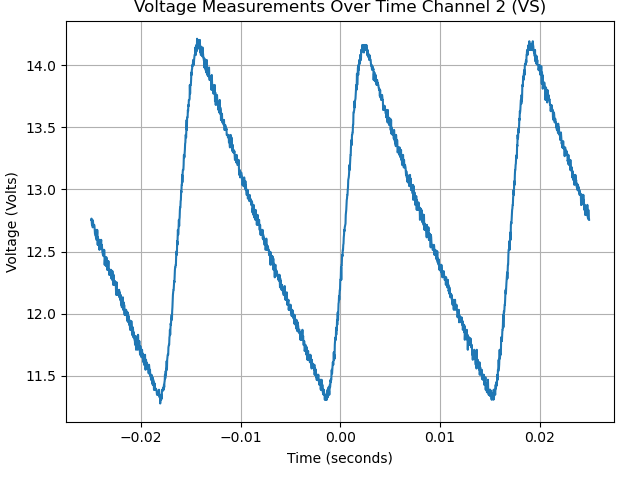
\includegraphics[width=\textwidth]{figures/F/4--ch2.png}
	    \caption{$V_S$ oscilloscope readout for \bref{exp::F}{Experiment F} $56\unit{\ohm}$ }
	\end{minipage}
\end{figure}
\begin{figure}[H]\label{data::F5}
	\centering
	\begin{minipage}[c]{0.45\textwidth}
		\centering
		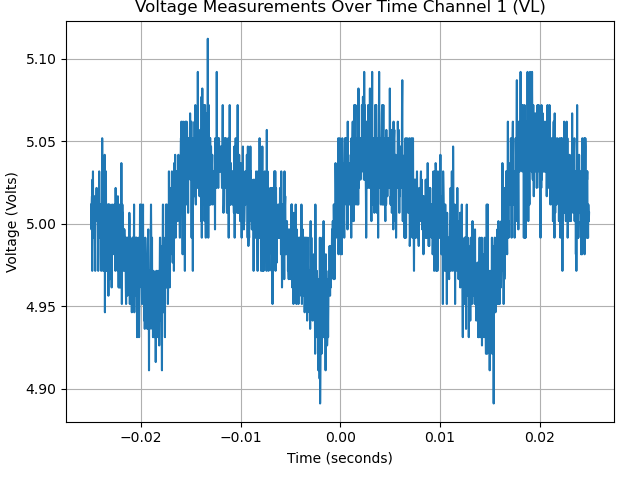
\includegraphics[width=\textwidth]{figures/F/5--ch1.png}
	    \caption{$V_L$ oscilloscope readout for \bref{exp::F}{Experiment F} $560\unit{\ohm}$ }
	\end{minipage}
	\hfill
	\begin{minipage}[c]{0.45\textwidth}
		\centering
		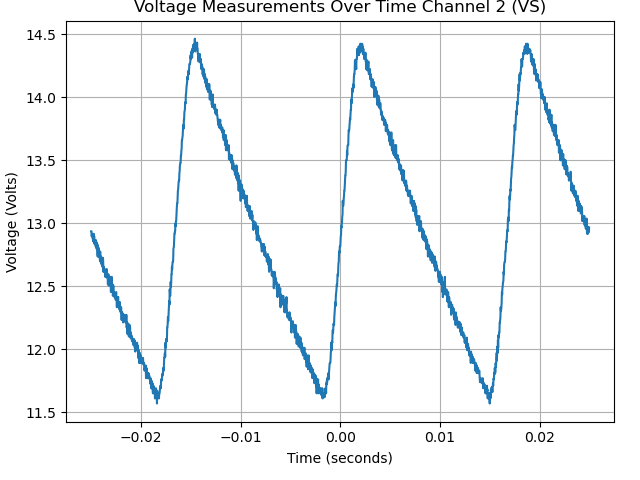
\includegraphics[width=\textwidth]{figures/F/5--ch2.png}
	    \caption{$V_S$ oscilloscope readout for \bref{exp::F}{Experiment F} $560\unit{\ohm}$ }
	\end{minipage}
\end{figure}
\begin{figure}[H]\label{data::F6}
	\centering
	\begin{minipage}[c]{0.45\textwidth}
		\centering
		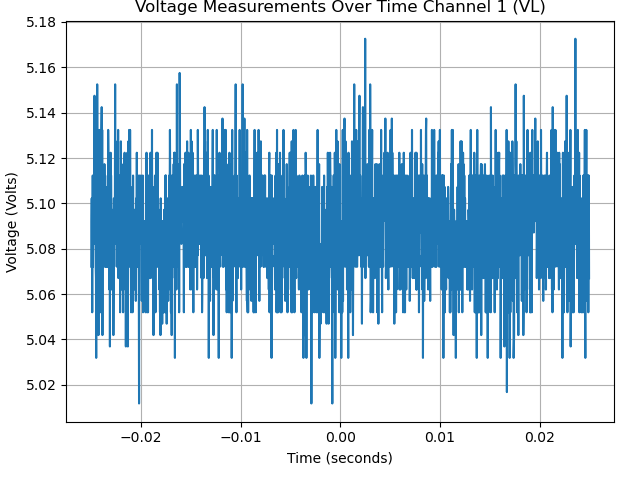
\includegraphics[width=\textwidth]{figures/F/6--ch1.png}
	    \caption{$V_L$ oscilloscope readout for \bref{exp::F}{Experiment F} $2.7\unit{k\ohm}$ }
	\end{minipage}
	\hfill
	\begin{minipage}[c]{0.45\textwidth}
		\centering
		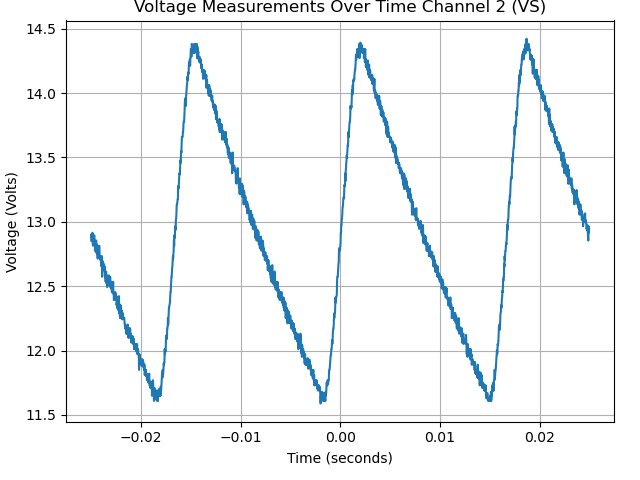
\includegraphics[width=\textwidth]{figures/F/6--ch2.png}
	    \caption{$V_S$ oscilloscope readout for \bref{exp::F}{Experiment F} $2.7\unit{k\ohm}$ }
	\end{minipage}
\end{figure}

\subsection{Experiment G}

\begin{figure}[H]\label{data::G}
	\centering
	\begin{minipage}[c]{0.45\textwidth}
		\centering
		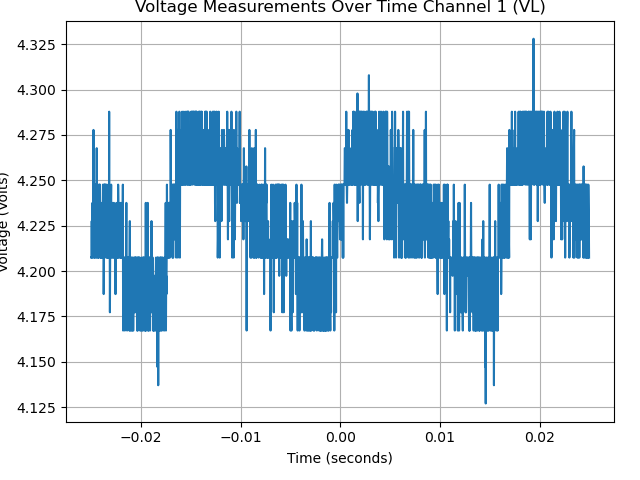
\includegraphics[width=\textwidth]{figures/G/1--ch1.png}
	    \caption{$V_{L}$ oscilloscope readout for \bref{exp::G}{Experiment G} $9.7\unit V$ }
	\end{minipage}
	\hfill
	\begin{minipage}[c]{0.45\textwidth}
		\centering
		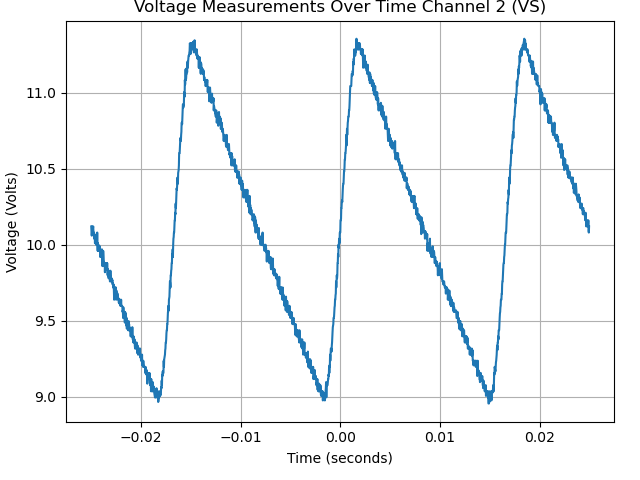
\includegraphics[width=\textwidth]{figures/G/1--ch2.png}
	    \caption{$V_{S}$ oscilloscope readout for \bref{exp::G}{Experiment G} $9.7\unit V$ }
	\end{minipage}
\end{figure}
\begin{figure}[H]\label{data::G2}
	\centering
	\begin{minipage}[c]{0.45\textwidth}
		\centering
		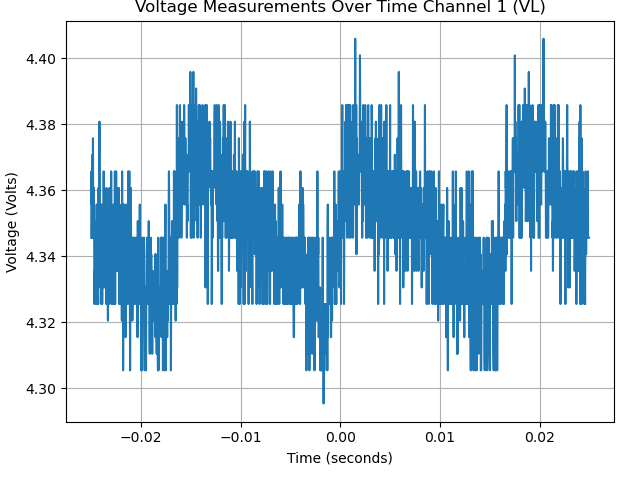
\includegraphics[width=\textwidth]{figures/G/2--ch1.png}
	    \caption{$V_{L}$ oscilloscope readout for \bref{exp::G}{Experiment G} $12.6\unit V$ }
	\end{minipage}
	\hfill
	\begin{minipage}[c]{0.45\textwidth}
		\centering
		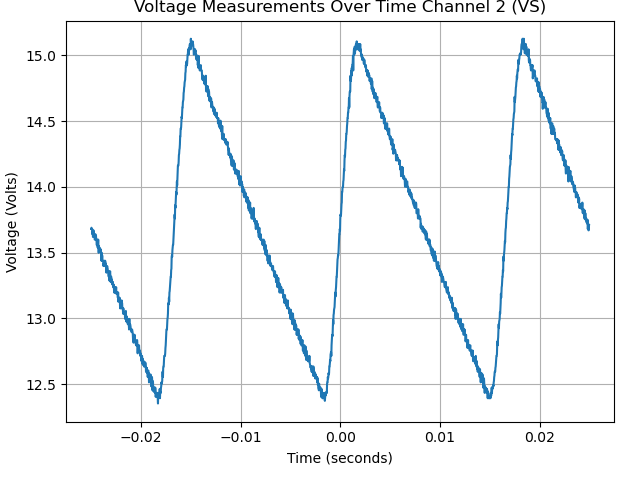
\includegraphics[width=\textwidth]{figures/G/2--ch2.png}
	    \caption{$V_{S}$ oscilloscope readout for \bref{exp::G}{Experiment G} $12.6\unit V$ }
	\end{minipage}
\end{figure}
\begin{figure}[H]\label{data::G3}
	\centering
	\begin{minipage}[c]{0.45\textwidth}
		\centering
		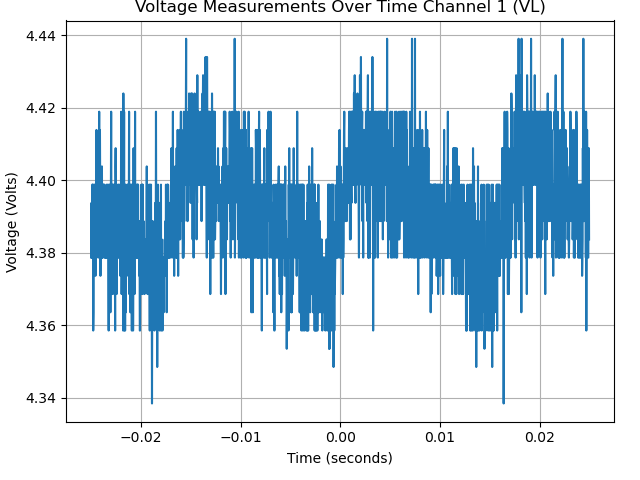
\includegraphics[width=\textwidth]{figures/G/3--ch1.png}
	    \caption{$V_{L}$ oscilloscope readout for \bref{exp::G}{Experiment G} $14.9\unit V$ }
	\end{minipage}
	\hfill
	\begin{minipage}[c]{0.45\textwidth}
		\centering
		\includegraphics[width=\textwidth]{figures/G/3--ch2.png}
	    \caption{$V_{S}$ oscilloscope readout for \bref{exp::G}{Experiment G} $14.9\unit V$ }
	\end{minipage}
\end{figure}
\begin{figure}[H]\label{data::G4}
	\centering
	\begin{minipage}[c]{0.45\textwidth}
		\centering
		\includegraphics[width=\textwidth]{figures/G/4--ch1.png}
	    \caption{$V_{L}$ oscilloscope readout for \bref{exp::G}{Experiment G} $56\unit{\ohm}$ }
	\end{minipage}
	\hfill
	\begin{minipage}[c]{0.45\textwidth}
		\centering
		\includegraphics[width=\textwidth]{figures/G/4--ch2.png}
	    \caption{$V_{S}$ oscilloscope readout for \bref{exp::G}{Experiment G} $56\unit{\ohm}$ }
	\end{minipage}
\end{figure}
\begin{figure}[H]\label{data::G5}
	\centering
	\begin{minipage}[c]{0.45\textwidth}
		\centering
		\includegraphics[width=\textwidth]{figures/G/5--ch1.png}
	    \caption{$V_{L}$ oscilloscope readout for \bref{exp::G}{Experiment G} $2.7\unit{k\ohm}$ }
	\end{minipage}
	\hfill
	\begin{minipage}[c]{0.45\textwidth}
		\centering
		\includegraphics[width=\textwidth]{figures/G/5--ch2.png}
	    \caption{$V_{S}$ oscilloscope readout for \bref{exp::G}{Experiment G} $2.7\unit{k\ohm}$ }
	\end{minipage}
\end{figure}
\subsection{Experiment H}
\begin{figure}[H]\label{data::H}
	\centering
	\begin{minipage}[c]{0.45\textwidth}
		\centering
		\includegraphics[width=\textwidth]{figures/H/1--ch2.png}
	    \caption{$V_{L}$ oscilloscope readout for \bref{exp::H}{Experiment H} $270\unit{\ohm}$ }
	\end{minipage}
	\hfill
	\begin{minipage}[c]{0.45\textwidth}
		\centering
		\includegraphics[width=\textwidth]{figures/G/2--ch2.png}
	    \caption{$V_{T}$ oscilloscope readout for \bref{exp::H}{Experiment H} $270\unit{\ohm}$ }
	\end{minipage}
\end{figure}
\begin{figure}[H]\label{data::H2}
	\centering
	\begin{minipage}[c]{0.45\textwidth}
		\centering
		\includegraphics[width=\textwidth]{figures/H/3--ch2.png}
	    \caption{$V_{T1}$ oscilloscope readout for \bref{exp::H}{Experiment H} $270\unit{\ohm}$ }
	\end{minipage}
	\hfill
	\begin{minipage}[c]{0.45\textwidth}
		\centering
		\includegraphics[width=\textwidth]{figures/H/4--ch2.png}
	    \caption{$V_{T2}$ oscilloscope readout for \bref{exp::H}{Experiment H} $270\unit{\ohm}$ }
	\end{minipage}
\end{figure}
\begin{figure}[H]\label{data::H3}
	\centering
	\begin{minipage}[c]{0.45\textwidth}
		\centering
		\includegraphics[width=\textwidth]{figures/H/5--ch2.png}
	    \caption{$V_{L}$ oscilloscope readout for \bref{exp::H}{Experiment H} $1\unit{k\ohm}$ }
	\end{minipage}
	\hfill
	\begin{minipage}[c]{0.45\textwidth}
		\centering
		\includegraphics[width=\textwidth]{figures/H/6--ch2.png}
	    \caption{$V_{T}$ oscilloscope readout for \bref{exp::H}{Experiment H} $1\unit{k\ohm}$ }
	\end{minipage}
\end{figure}
\begin{figure}[H]\label{data::H4}
	\centering
	\begin{minipage}[c]{0.45\textwidth}
		\centering
		\includegraphics[width=\textwidth]{figures/H/7--ch2.png}
	    \caption{$V_{T1}$ oscilloscope readout for \bref{exp::H}{Experiment H} $1\unit{k\ohm}$ }
	\end{minipage}
	\hfill
	\begin{minipage}[c]{0.45\textwidth}
		\centering
		\includegraphics[width=\textwidth]{figures/H/8--ch2.png}
	    \caption{$V_{T2}$ oscilloscope readout for \bref{exp::H}{Experiment H} $1\unit{k\ohm}$ }
	\end{minipage}
\end{figure}
\begin{figure}[H]\label{data::H5}
	\centering
	\begin{minipage}[c]{0.45\textwidth}
		\centering
		\includegraphics[width=\textwidth]{figures/H/9--ch2.png}
	    \caption{$V_{L}$ oscilloscope readout for \bref{exp::H}{Experiment H} $2.7\unit{k\ohm}$ }
	\end{minipage}
	\hfill
	\begin{minipage}[c]{0.45\textwidth}
		\centering
		\includegraphics[width=\textwidth]{figures/H/10--ch2.png}
	    \caption{$V_{T}$ oscilloscope readout for \bref{exp::H}{Experiment H} $2.7\unit{k\ohm}$ }
	\end{minipage}
\end{figure}
\begin{figure}[H]\label{data::H6}
	\centering
	\begin{minipage}[c]{0.45\textwidth}
		\centering
		\includegraphics[width=\textwidth]{figures/H/11--ch2.png}
	    \caption{$V_{T1}$ oscilloscope readout for \bref{exp::H}{Experiment H} $2.7\unit{k\ohm}$ }
	\end{minipage}
	\hfill
	\begin{minipage}[c]{0.45\textwidth}
		\centering
		\includegraphics[width=\textwidth]{figures/H/12--ch2.png}
	    \caption{$V_{T2}$ oscilloscope readout for \bref{exp::H}{Experiment H} $2.7\unit{k\ohm}$ }
	\end{minipage}
\end{figure}
\bibliographystyle{apacite}
\bibliography{references.bib}
\end{document}
